\documentclass[12pt,a4paper,notitlepage]{article}
\usepackage[utf8]{inputenc}
\usepackage[english]{babel}
\usepackage[T1]{fontenc}
\usepackage[backend=biber,
			style=authoryear-comp,
			isbn=false,
			doi=false,
			bibstyle=authoryear,
			natbib,
			]{biblatex}
\usepackage{eurosym}
\usepackage{enumitem}
\usepackage{url}
\usepackage{blindtext}
\usepackage{hyperref}
\usepackage{breakurl}
\usepackage{amsmath}
\usepackage{titling}
\usepackage{amsfonts}
\usepackage{amssymb}
\usepackage{pgfplots}
\usepackage{caption}
\usepackage{subcaption}
\usepackage{graphicx}
\usepackage{dcolumn}
\usepackage{tikz-3dplot}
\usepackage{subcaption}
\usepackage{float}
\usepackage{adjustbox}
\usepackage{multirow,rotating}
\usepackage[autostyle]{csquotes}
\usepackage[toc,page]{appendix}
\usepackage{lscape}
\usepackage{todonotes}
\usepackage{booktabs}
\usepackage{multirow}
\usepackage{bm}
\usepackage{eurosym}
\usepackage{pdflscape}

\addbibresource{Textmining.bib}

\title{Topic and tone of political news articles in German online media.}
\date{\today}
\author{Franziska Löw}

\begin{document}
\begin{titlepage}
	\maketitle
	\begin{abstract}
		The aim of this paper is to investigate whether the political reporting of different content providers distinguishes itself and whether this reporting has an influence on the opinion-forming process of the voters. 
		
		\textbf{Keywords} Structural Topic Model, Sentiment Analysis, Unsupervised Machine Learning, Text Mining

	\end{abstract}

\end{titlepage}

\section{Introduction}
% Noch deutlicher beschreiben, was eigentlich gemacht wird. Besser motivieren
% Paper von Ralf, Melissa, Tobias zitieren. 

Pluralism is an essential principle of democratic societies. An important pillar of this principle is an opinion-forming process that incorporates the different perspectives represented in the society. For the process of forming opinions, information conveyed by the media, in particular the mass media of journalism, plays a decisive role. They create the preconditions for making the social and cultural diversity of modern societies visible and manageable. Securing the diversity of opinion-forming processes and preventing concentration processes in the media sector is an essential prerequisite for a functioning democracy. An important question is therefore whether the political reporting of different content providers distinguishes itself and whether this reporting has an influence on the opinion-forming process of the voters. The aim of this paper is to investigate these questions with the use of up-to-date text mining methods.  

A number of different factors have an influence on the diversity of media content. These include the market structure for journalistic content and the digitization of the industry. Media outlets (TV, Radio, Newspaper) usually operate in two-sided markets, where they serve two customer groups (content consumer and advertiser) that are connected via indirect network effects. The two-sided market structure of the private news market results in news platforms striving to choose their content in such a way that its reach is as large as possible in order to maximize profits from advertising revenues. \citet{steiner_program_1952} concluded, that profit-maximizing media owners may choose to offer the same content, i.e. content aligned with the tastes of the majority. \citet{gabszewicz_press_2001} study the problem of diversity of the political content of newspapers. They find that the maximum differentiation only prevails if the readers sufficiently value the political differentiation between the newspapers the advertising market is small enough. On the other hand, advertising may also have a positive impact on the media, as it enables publishers to report independently of political parties. \citet{ellman_what_2009} analyze a theoretical framework of a two-sided market for newspaper, where readers value accuracy and advertisers value advert-receptive readers. They found that advertising increases the intensity of competition for readers and therefore raises accuracy of media coverage. However, in the monopolistic case, newspapers under-report news that sufficiently reduces advertiser profits. 

The new developments in digital media provide new opportunities and challenges for media outlets. The costs of providing and disseminating information have been reduced and the speed of information exchange has increased enormously. At first glance, these developments seem to have a positive effect on the provision of information. However, it also means that the incentive for media to produce primary information declines since the Internet has reduced the marginal utility of content. A study of French news websites from 2013 shows that only 38 percent of the online articles contained original content, with the remainder being copies of those originals \citep{cage_information_2017}. At the same time, the number of people who find out about current news on the Internet is increasing. According to a study on the media coverage of the German-speaking population, nearly 40\% of respondents used the internet at least once a week in 2017 to inform themselves about the current news compared to 34\% in 2016 \citep{vuma_arbeitsgemeinschaft_verbrauchs-_und_medienanalyse_verbrauchs-_2017}. Recognizing the importance of media pluralism, the European Commission has endorsed several initiatives to discuss and promote media diversity in the European Union\footnote{https://ec.europa.eu/digital-single-market/en/policies/media-freedom-and-pluralism}. One way to ensure the independence and diversity of the media landscape is through public funded media. In Germany public broadcasting originated in the post-war period and is financed by compulsory fees. To take into account the distinct nature of digital media, the Interstate Broadcasting Agreement (Rundfunkstaatsvertrag) also regulates the scope for action of online services offered by public service broadcasting since 2007. Accordingly, public media are not allowed to distribute purchased content and must - depending on the category of content - set a time limit on its accessibility. In addition, there is a strict advertising ban and prohibition of regional reporting. 

With the purpose of examining the media pluralism in the market for German-language online news, this paper analyzes German online news articles about domestic politics. German federal elections took place on 24th of September 2017 and the formation of the government has taken up a period of about five month. The articles considered here dated from 01.06.2017 to 01.03.2018 and thus inform their readers both about the election promises of the parties (before the election) and about the coalition talks (after the election). They therefore make an important contribution to the public's opinion-forming process. The empirical strategy follows a novel approach combining "the two Ts": Topic and Tone \citep{hansen_shocking_2016}. That is, first the topics covered in the articles are identified, to find out how these topics are discussed (tone). The final step is to check whether the tonality of reporting is reflected in the survey results on voting preferences calculating the cross-correlation coefficients. More precisely, the research strategy is as follows:

\begin{enumerate}
	\item\label{item_1} \textbf{Discovering Topics (Section \ref{subsection_topic})} To discover the latent topics in the corpus, the structural topic modeling (STM) developed by \citet{roberts_model_2016} is applied. The STM is an unsupervised machine learning approach that models topics as multinomial distributions of words and documents (as a synonym for news articles) as multinomial distributions of topics, allowing to incorporate external variables that effect both, topical content and topical prevalence. I estimate a model, where the newswire service is included as a control for both the topical content and the topical prevalence. The result of the generative process of STM are the posterior distributions for topic prevalence in a document and the content of a topic. The latter is used to label the topics according to an event or issue discussed in the media. The probability distribution of topics for each document is used to assign a topic to each news article. 
	\item\label{item_2} \textbf{Measuring Tone (Section \ref{subsection_tone})} After assigning a topic to each article (document), a dictionary-based sentiment analysis is conducted to estimate how topics are discussed differently by different news wires.
	\item\label{item_3} \textbf{Comparing with polls} In order to check whether the transmitted content from the online media is reflected in the voting preferences, we compare the values from \ref{item_2} with the survey values of the Sunday survey ("Sonntagsumfrage").

% Der erste Absatz ist z.B. ziemlich knapp. Ebenso sind „Measuring Tone“ und „Comparing with polls“ sehr knapp im Vergleich zu „Dicovering topics“ beschrieben.

\end{enumerate}

Approach \ref{item_1} has been used in \citet{roberts_model_2016}, among others, to examine differences in the content of eastern and western news providers regarding "the rise of China". However, I extend the analysis by comparing the sentiment score for a given topic an news provider, to identify which topics are discussed similar or differently (\ref{item_2}). \citet{hansen_shocking_2016} applied a similar approach to a dataset of 142 FOMC decision statements to measure the effect of those statements on macroeconomic variables. An additional extension is the comparison with current election poll values (\ref{item_3}). 

The remaining course of the paper is as follows: The following Section \ref{ch_elections} gives an overview about political trends in the past six month (June 2017 to March 2018). The data used to conduct the model is described in Section \ref{ch_data}. Section \ref{ch_model} explains the generative process of the structural topic model as well as the selected parameters to run the model. The empirical analysis containing the above mentioned steps is conducted in Section \ref{ch_empirical}. 
 
% -------------------------
% Background Bundestagswahl
% -------------------------
\section{Background on the federal election in Germany (2017)}\label{ch_elections}

The articles analyzed in this paper cover a period from June 1, 2017 to March 1, 2018 and thus cover both the most important election campaign topics for the Bundestag elections on September 24, 2017 and the process of forming a government that lasted until February 2018. After four years in a grand coalition with the Social Democrats (SPD), German Chancellor Angela Merkel, member of the Conservative Party (CDU), ran for re-election. The SPD nominated Martin Schulz as candidate for chancellor. 

On the right side of the political spectrum, AfD (alternative for Germany) managed to be elected to the German Bundestag for the first time in 2017. The political debate about the high refugee numbers of the past years brought the AfD a political upswing by taking up the dissatisfaction of parts of the population and using it to raise its own profile. Leading party members of the AfD as well as party supporters repeatedly accused the mass media in the course of the reporting on the federal elections to report unilaterally and to present the AfD intentionally badly.

After the election, the formation of a government was difficult due to the large number of parties elected to the Bundestag and the considerable loss of votes by the major parties CDU/CSU and SPD. Since all parties rejected a coalition with the AfD, numerically only two coalitions with an absolute parliamentary majority were possible: a grand coalition ("GroKo") of CDU/CSU and SPD, and a Jamaica coalition (coalition of CDU/CSU, FDP (economic liberal party) and B90/Die Grünen (Bündnis 90/Die Grünen, green party)). The grand coalition was initially rejected by the SPD. The four-week exploratory talks on the possible formation of a Jamaica coalition officially failed on 19 November 2017 after the FDP announced its withdrawal from the negotiations. FDP party leader Christian Lindner said that there had been no trust between the parties during the negotiations. The main points of contention were climate and refugee policy. CDU and CSU regretted this result, while B90/Die Grünen sharply criticized the withdrawal of the Liberals. The then Green leader Cem Özdemir accused the FDP of lacking the will to reach an agreement.

After the failure of the Jamaica coalition, a possible re-election or a minority government as alternatives were discussed in the media before the SPD decided to hold coalition talks with the CDU/CSU. This led to great resistance from the party base, which called for a party-internal vote on a grand coalition. After the party members voted in favor of the grand coalition, a government was formed 171 days after the federal elections. 

Figure \ref{fig_polls} shows that support for the two major popular parties has been declining in recent months since August 2017, with the CDU again showing positive survey results since November. However, the value of the SPD has been falling since March 2017. At the same time, the AfD in particular has been recording increasingly positive survey results since June 2017. Section \ref{ch_correlation} examines whether there is a correlation between the survey results and the way the parties are reported in the media. 

\begin{figure}[H]
\begin{center}
	\caption{Election Polls}
	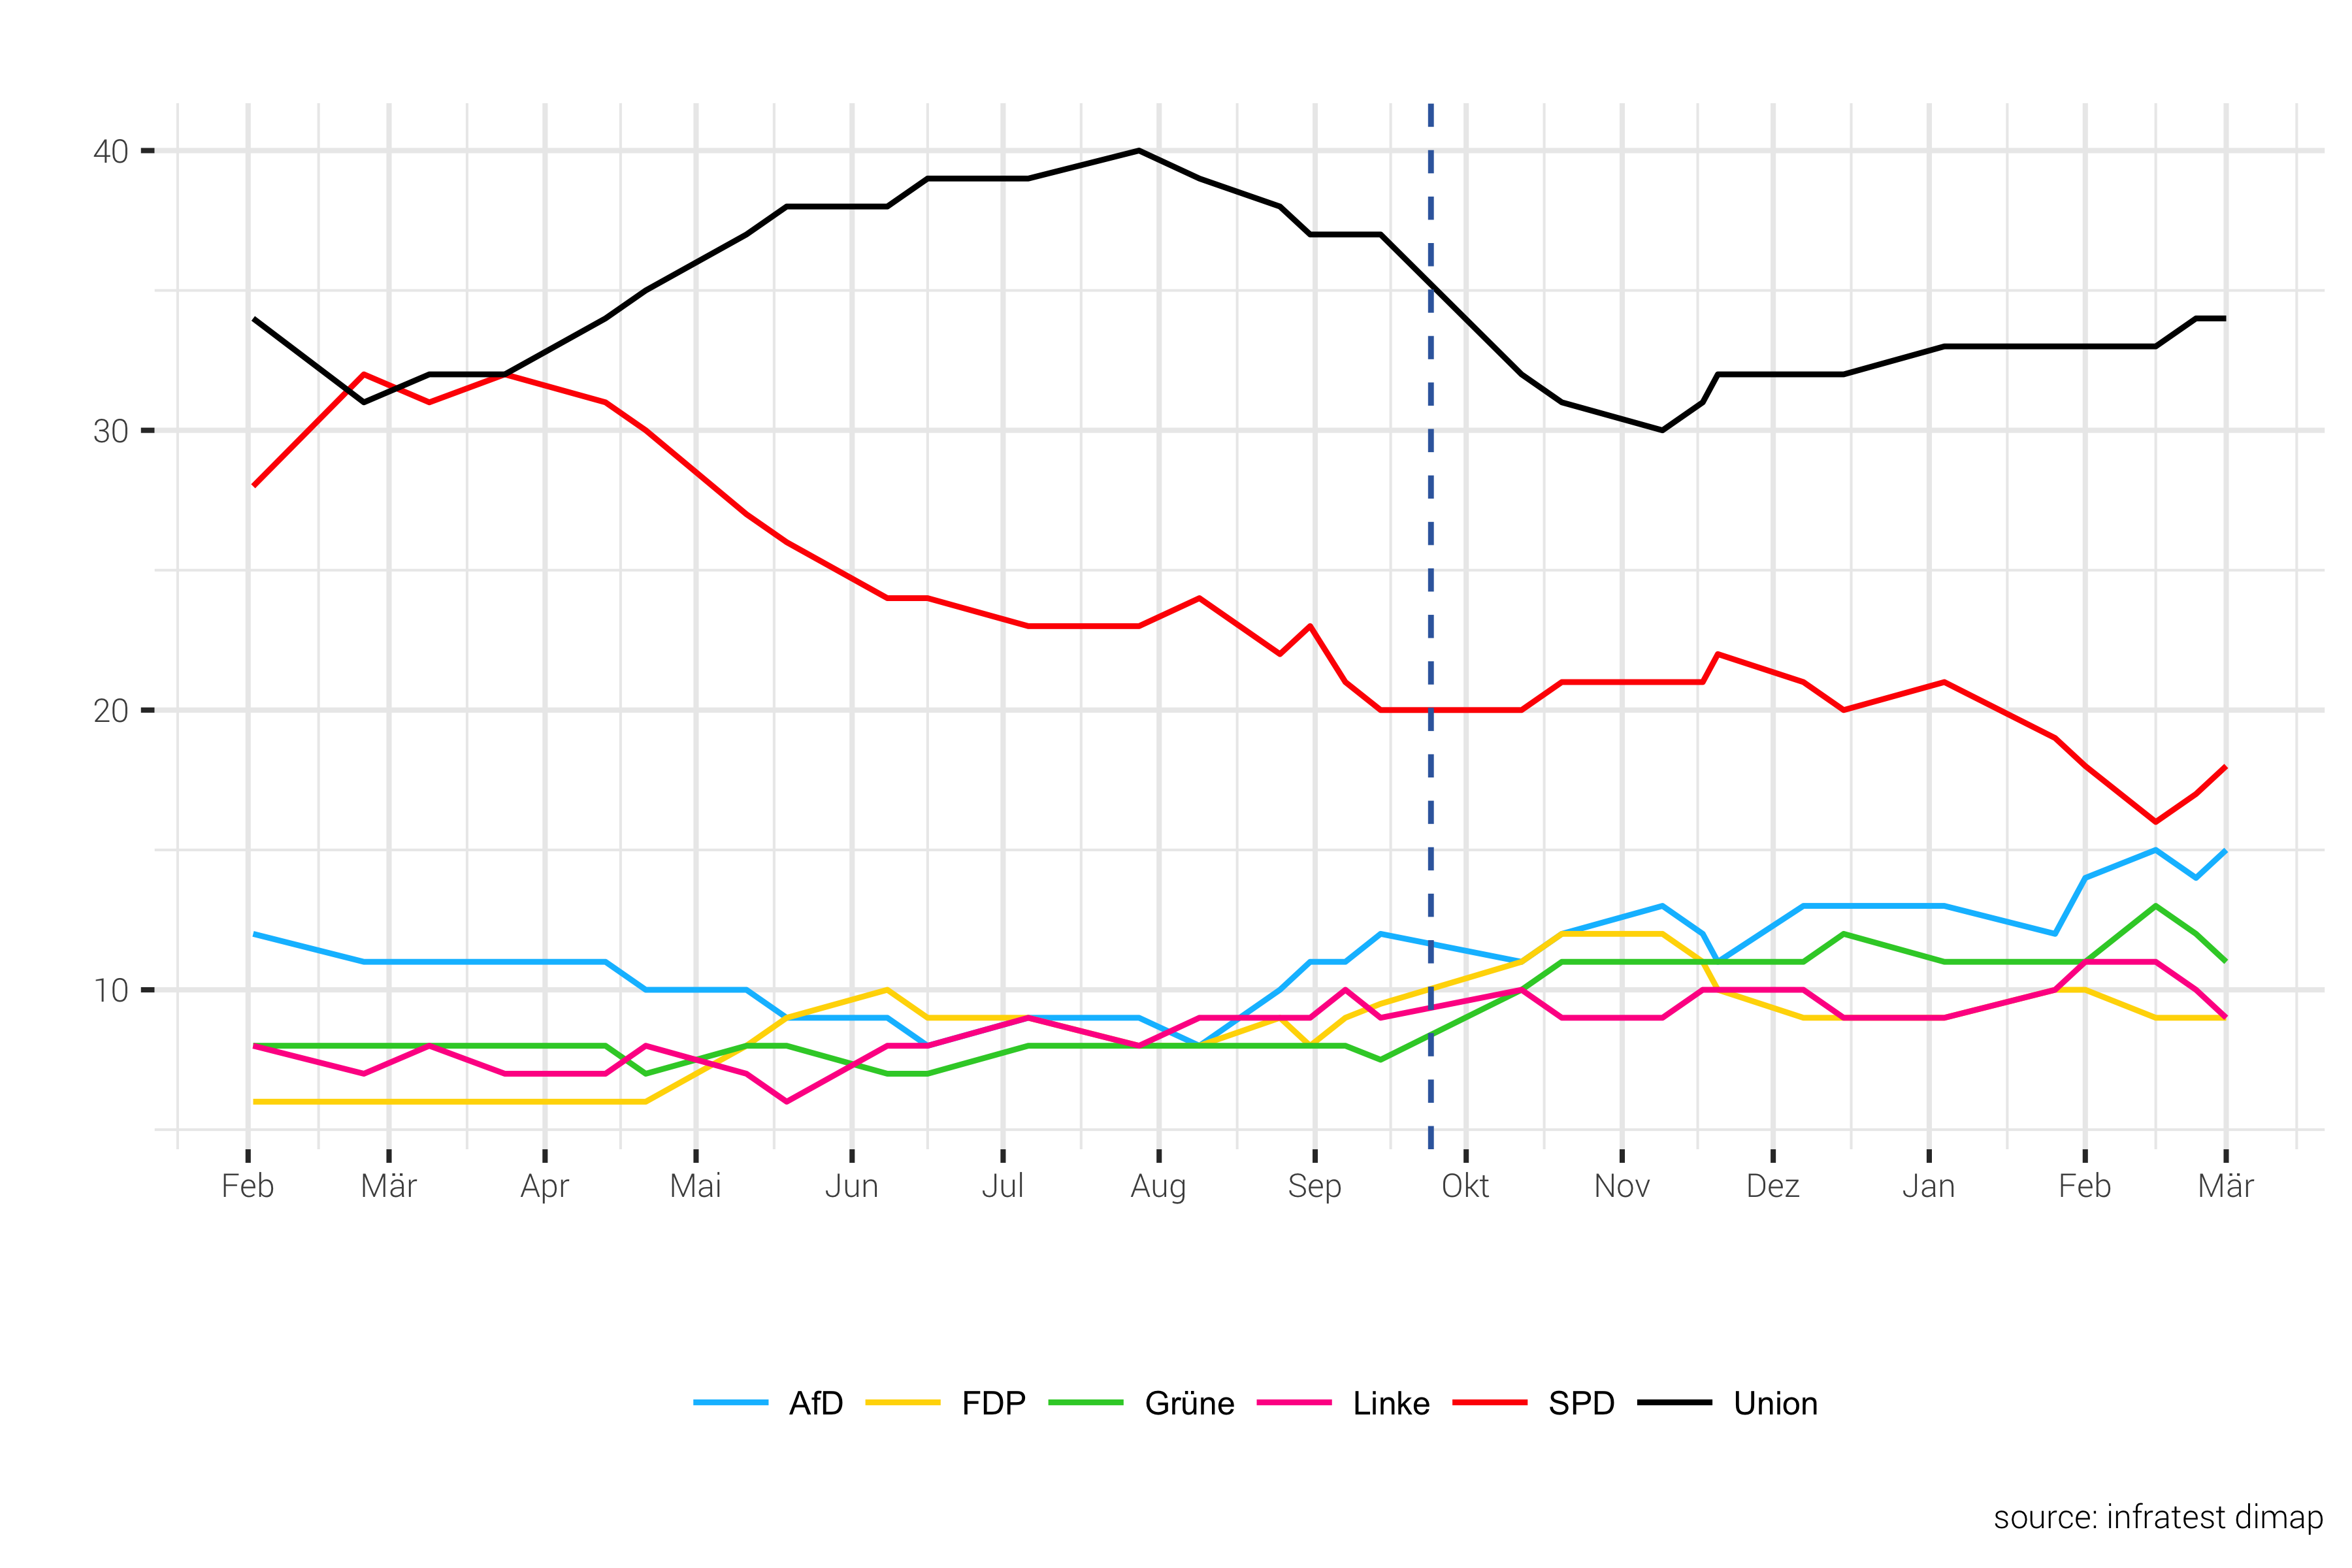
\includegraphics[width=0.8\textwidth]{../figs/polls.png}
	\label{fig_polls}
	\end{center}
\end{figure}

% -----
% Data
% -----
\section{Dataset and data preparation}\label{ch_data}
% Viel mehr Datenbeschreibung / deskriptive Statistik
% Warum wurden grade diese Medien ausgesucht?

I conduct the estimation on a sample of 14,937 online news articles from seven german news provider about domestic politics\footnote{Bild.de, DIE WELT, FOCUS ONLINE, SPIEGEL ONLINE, stern.de, ZEIT ONLINE, Tagesschau.de}. The articles are dated from 01.06.2017 to 01.03.2018. I first extract all online articles using the the Webhose.io API.\footnote{For more information see https://docs.webhose.io/v1.0/docs/getting-started. The scraping code was written in Python and can be made available on request.} Then all articles from the section "domestic policy" are filtered by using the URL of an article. Figure \ref{fig_distr1} shows the distribution of the number of articles from the respective news sources by date. There is a high peak around the federal elections on September, 24th.  

\begin{figure}[H]
	\caption{Article distribution...}
	\begin{center}
		\begin{subfigure}[normla]{0.49\textwidth}
			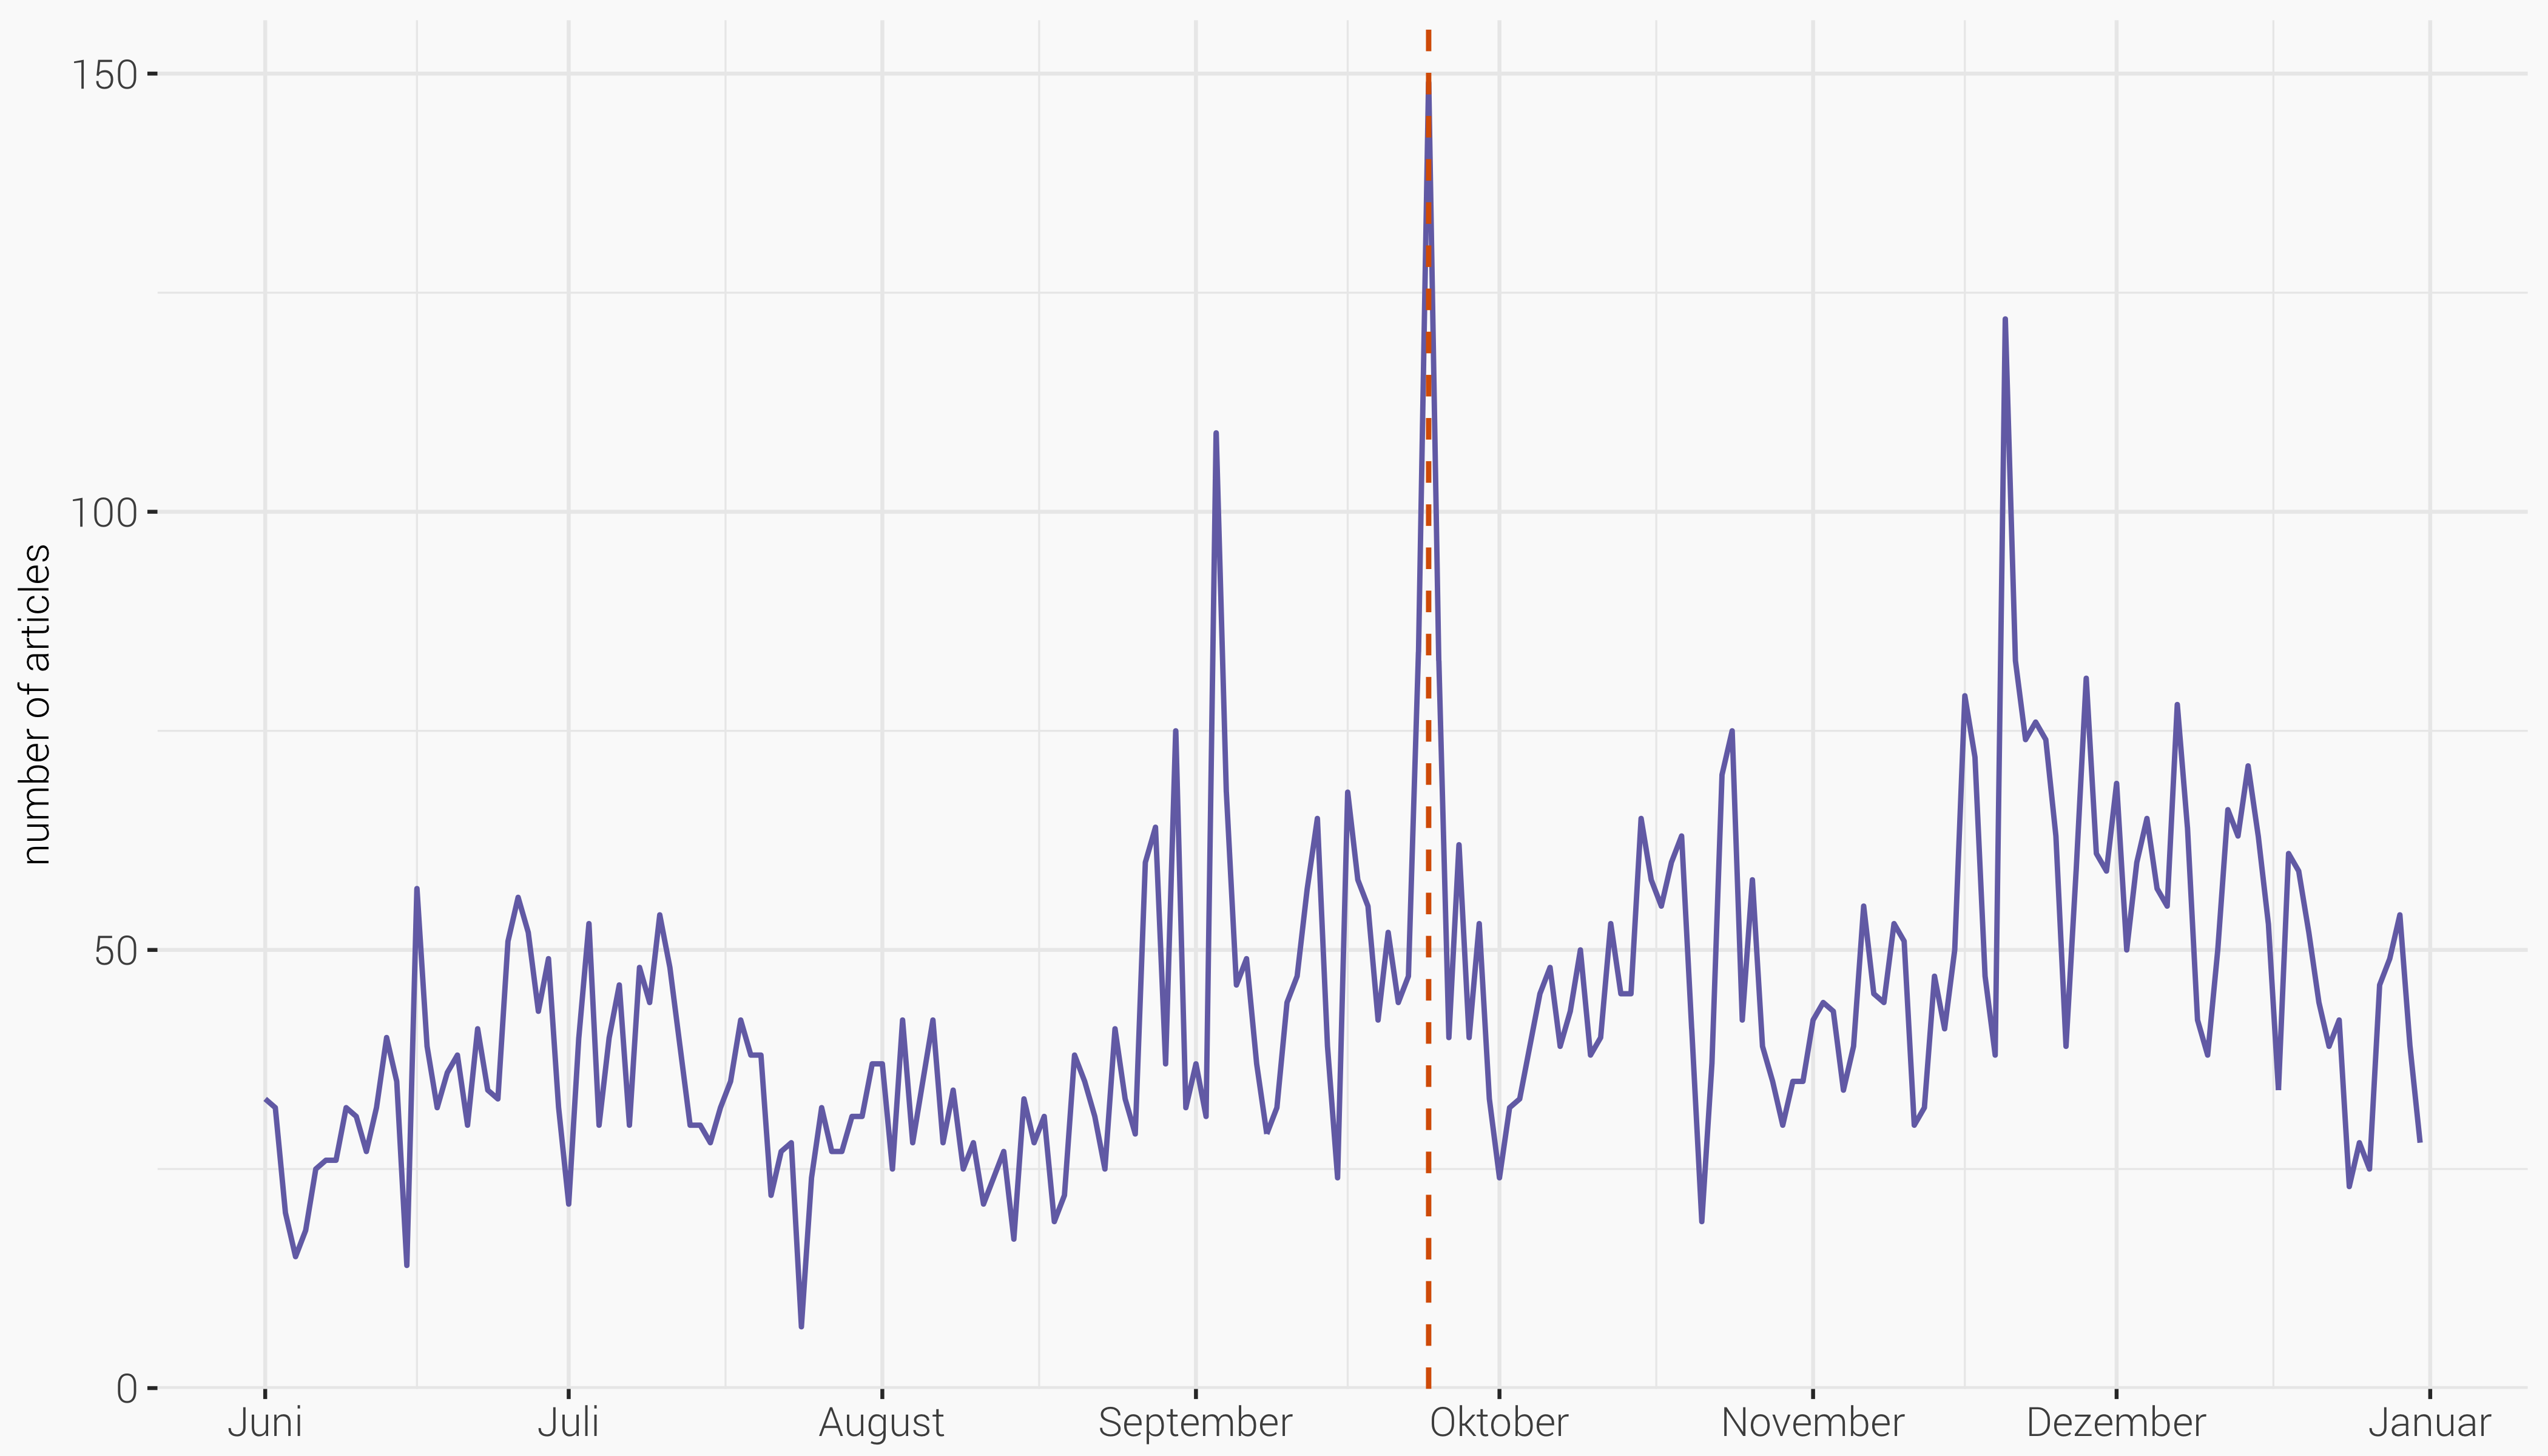
\includegraphics[width=\textwidth]{../figs/timeline.png}
			\caption{...by date}
			\label{fig_distr1}
		\end{subfigure}
		\begin{subfigure}[normla]{0.49\textwidth}
			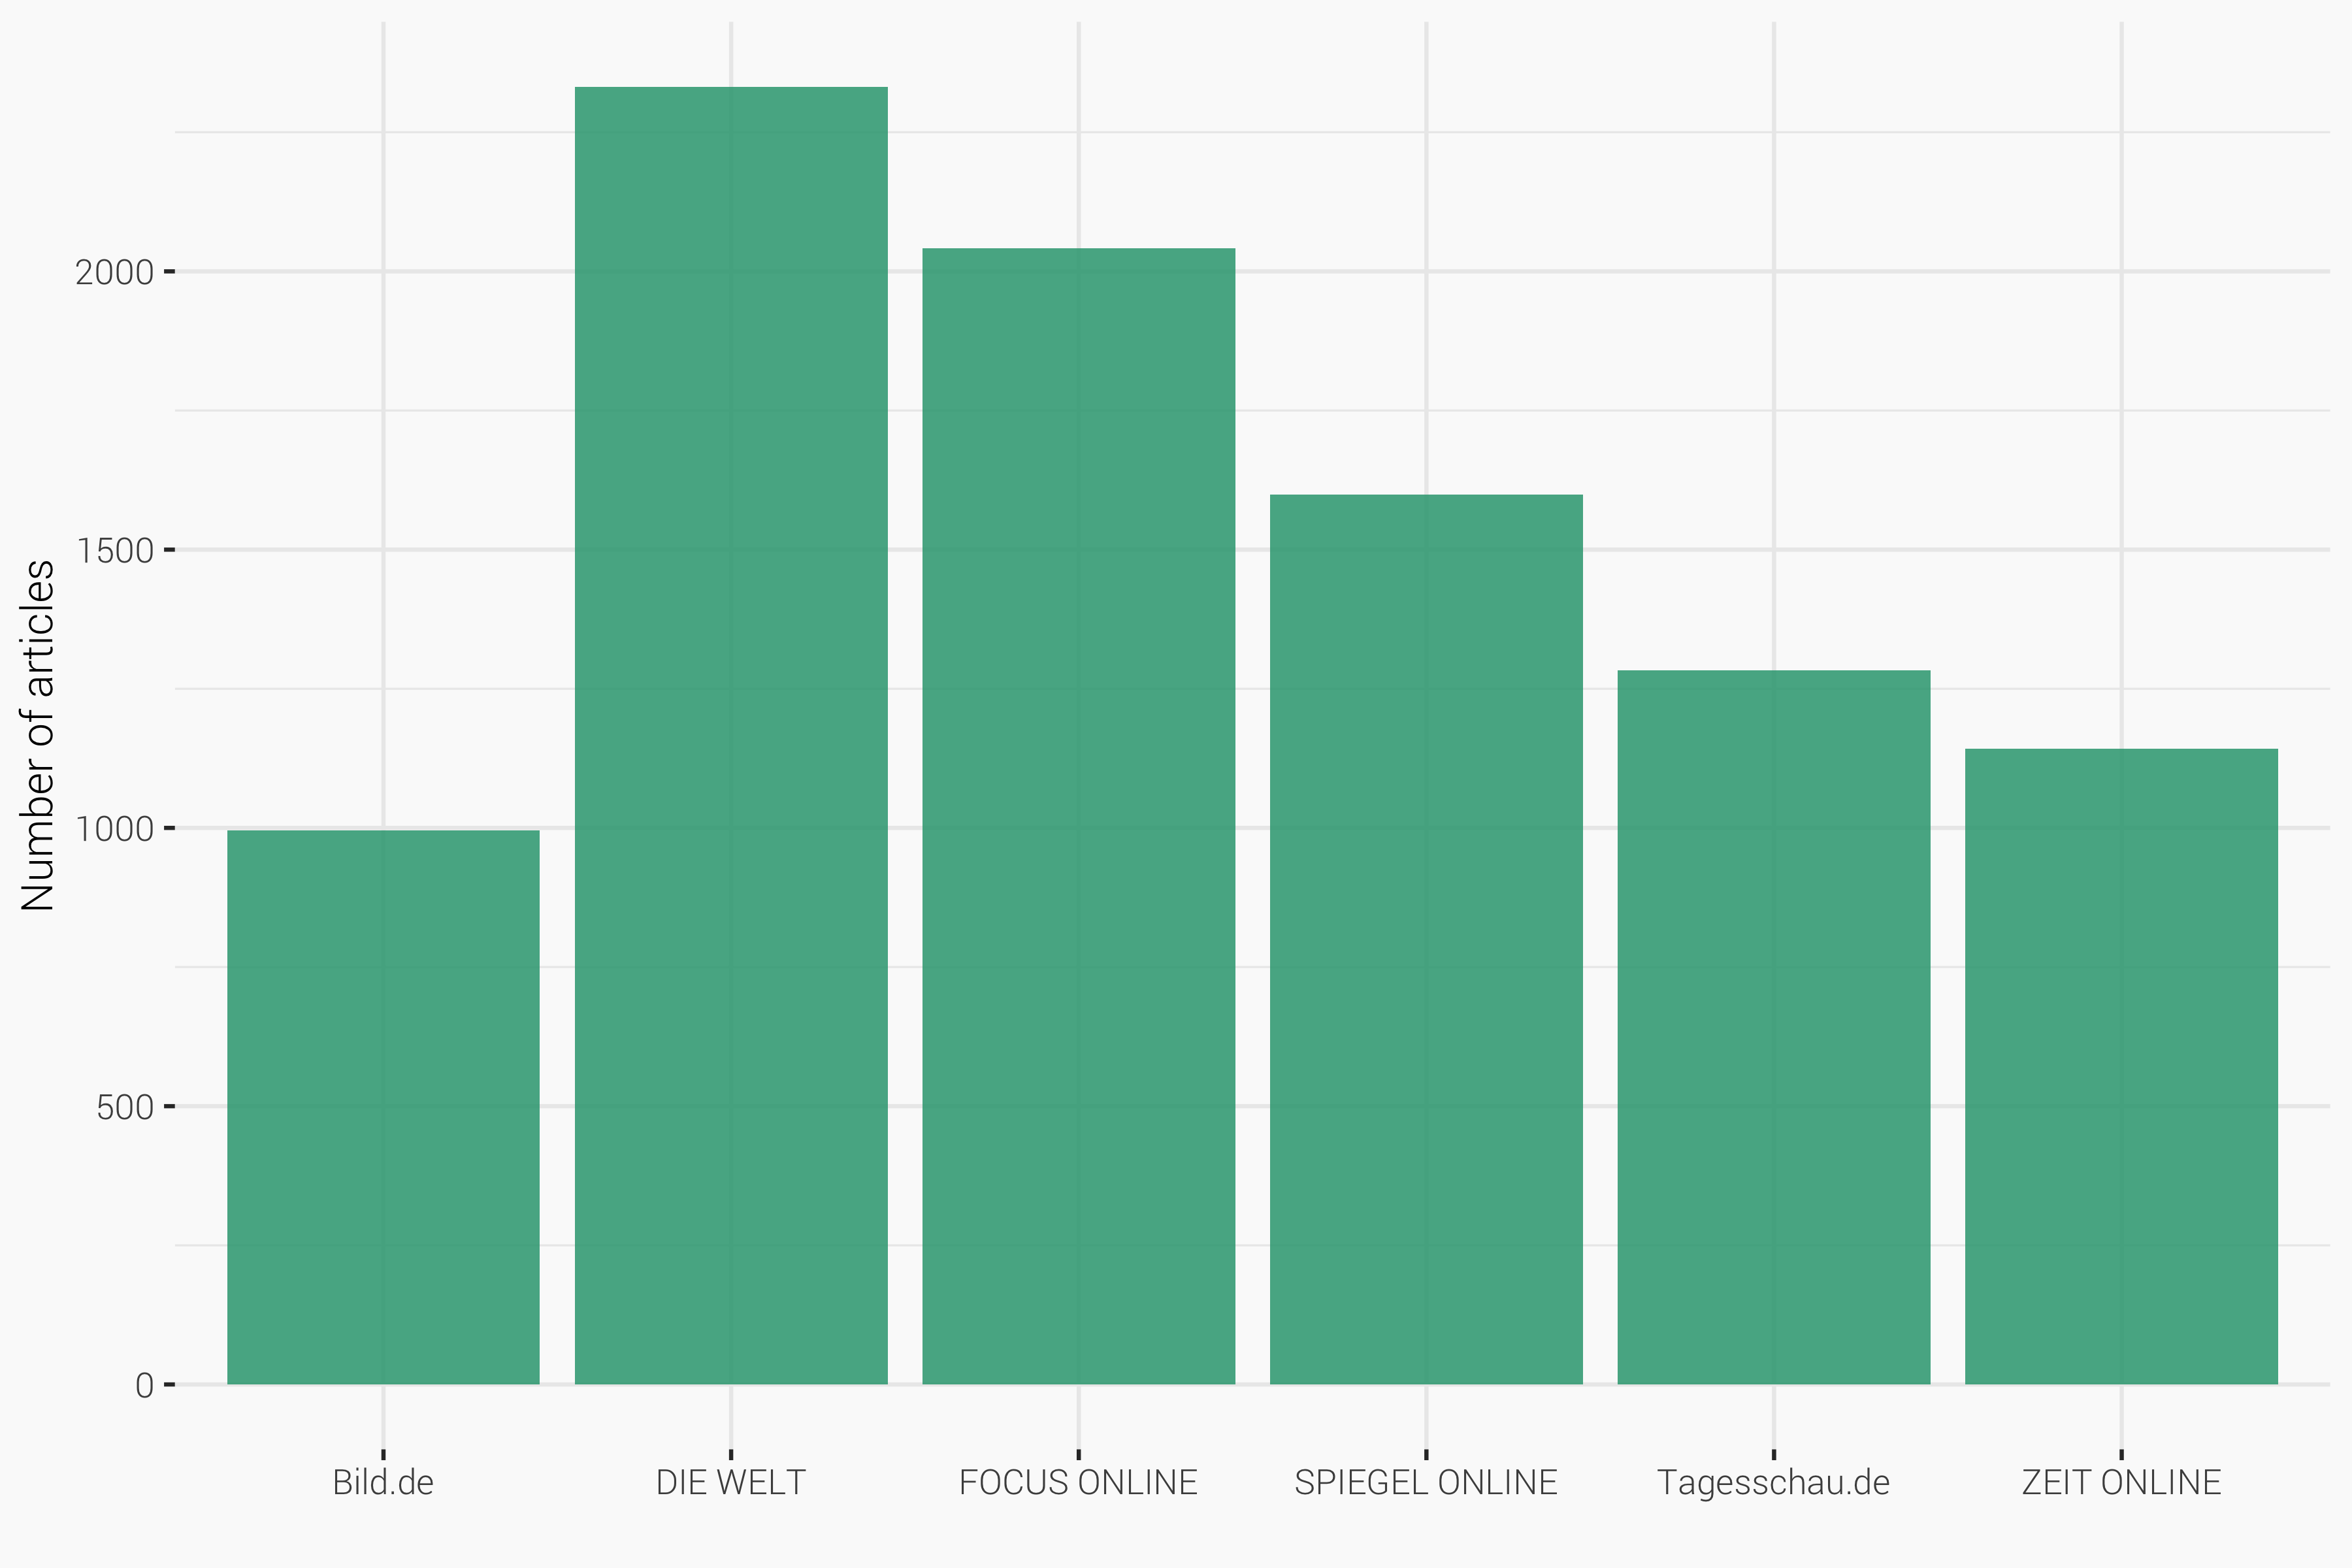
\includegraphics[width=\textwidth]{../figs/bar.png}
			\caption{... by news source}
			\label{fig_distr2}
		\end{subfigure}
	\end{center}
\end{figure}

Overall, the selected news providers are among the top ten German online news providers in the period under review, with only Tagesschau.de belonging to the public media. The reason for this is that the content structure of Tagesschau.de is most similar to that of the private providers. ZDF.de offers predominantly video content and DLF website mainly offers audio content in the form of interviews, which makes it hard to include it in the model. 


% ------------------
% Text Pre-Procesing
% ------------------
% Mehr beschreiben was hier gemacht wird. Was ist z.b. eine stop-word list? 

A central task in text mining is to extract low-dimensional information from documents that are high-dimensional by nature \citep{bholat_text_2015}. This is related to the task of reducing the number of unique language elements in order to reduce the dimensionality of data (to avoid unnecessary computational complexity and overfitting) while at the same time keeping those words that reflect the content of a document. Any useful representation of text will throw away some information, the trick is to include the relevant information that is needed, and exclude the extraneous information. A common strategy to use text as data and reduce the dimensionality, is to pre-process the text by imposing some preliminary restrictions (stop-word removal, tokenization) based on the nature of the data (twitter text, newspaper articles, speeches, etc.) to reduce the number of language elements \citep{gentzkow_text_2017}. 

Intuitively the term frequency (tf) of a word is a measure of how important that word may be. There are words in a document, however, that occur many times but may not be important like articles, conjunctions, and so on. These terms, often called "stop words", are important to the grammatical structure of a text, but typically don't add any additional meaning and can therefore be neglected. We use a pre-defined stop word list from the Snowball stemmer project\footnote{http://svn.tartarus.org/snowball/trunk/website/algorithms/*/stop.txt} together with a customized list of stop-words that are redundant superfluous or distorting. We also remove punctuation character (e.g. ., ,, !, ?, etc.) and all numbers from our corpus. After completing this steps we were left with 68.576 unique terms in our vocabulary.

After pre-processing, each document $d$ is a finite list of terms. Each unique term in the corpus is indexed by some $v \in \lbrace 1,...,V \rbrace$ where $V$ is the number of unique terms. For each document $d \in \lbrace 1,...,D \rbrace$ we compute the number of occurrences of term $v$ in document $d$ to obtain the count $x_{d,v}$. The $D$ x $V$ matrix $\boldsymbol{X}$ of all such counts is called the document-term matrix. This representation is often referred to as the bag of words model, since the order in which words are used within a document is completely disregarded. 

% ----------------------
% Structural topic Model
% ----------------------
\section{The structural topic model}\label{ch_model}
% Kapitel mehr mit eigenen Worten beschreiben. 

The structural topic model (STM) developed by \citet{roberts_model_2016} allows to incorporate document specific covariates (e.g. the author or date of a document). STM is a recent extension of the standard topic modeling technique, labeled as "latent Dirichlet allocation" (LDA), which refers to the Bayesian model in \citet{blei_latent_2003} that treats each word in a topic and each topic in a document as generated from a Dirichlet - distributed prior.\footnote{See also \citet{griffiths_probabilistic_2002}, \citet{griffiths_finding_2004} and \citet{hofmann_probabilistic_1999}. \citet{pritchard_inference_2000} introduced the same model in genetics for factorizing gene expression as a function of latent populations.} Topic models formalize the idea that documents are formed by hidden variables (topics) that generate correlations among observed terms. Since its introduction into text analysis, LDA has become hugely popular and especially useful in political science.\footnote{see \citet{blei_probabilistic_2012}, \citet{grimmer_text_2013} and \citet{wiedmann_text_2016} for an overview in social science and \citet{gentzkow_text_2017} give an overview of text mining applications in economics.} \citet{wiedmann_text_2016} uses topic model methods on large amounts of news articles from two german newspapers published between 1959 and 2011, to reveal how democratic demarcation was performed in Germany over the past six decades. \citet{paul_cross-collection_2017} compares editorial differences between media sources, using cross-collection latent Dirichlet allocation (ccLDA), an LDA-based approach that incorporates differences in document metadata. They use a dataset of 623 news articles from August 2008 from two American media outlets - msnbc.com and foxnews.com - to compare how they discuss topics. Reviewing the top words of the word-topic distribution, they find some content differences between the two. 

STM has been applied to multiple academic fields: \citet{roberts_structural_2014} uses STM to analyze open-ended responses from surveys and experiments, \citet{farrell_corporate_2016} applies the model to scientific texts on climate change, revealing links between corporate funding and the framing of scientific studies. \citet{mishler_using_2015} show that "STM can be used to detect significant events such as the downing of Malaysia Air Flight 17" when applied to twitter data. Another study shows how STM can be used to explore the main international development topics of countries’ annual statements in the UN General Debate and examine the country-specific drivers of international development rhetoric \citep{baturo_what_2017}. \citet{mueller_reading_2016} use newspaper text to predict armed conflicts in different regions. They use the estimated topic shares in linear fixed effects regression to forecast conflict out-of-sample. \citet{roberts_navigating_2016} use STM to examine the role of partisanship in topical coverage using a corpus of 13,246 posts that were written for 6 political blogs during the course of the 2008 U.S. presidential election. With the aim of revealing the effect of partisan membership on topic prevalence, each blog is assigned to be either liberal or conservative. To explore the differences between the two, they look at the expected proportion of topic and examine the posts most associated with a respective topic. This approach is similar to \citet{roberts_model_2016}. They also use different measures of distance between the topic-word distributions of the same topic within different models.

% Topic Modeling
% --------------
\subsection{Generative Process of STM}\label{ch_generativeProcess}

As mentioned above, the STM allows to incorporate observed document metadata which is able to affect both topical prevalence and topical content. The following description of the generative model - the process of filling a word-position in a document - of the STM is based on \citet{roberts_structural_2013} and \citet{roberts_stm:_2016}. For each document $d$ and a given number of topics $K$, a document-specific topic-prevalence vector $d(\boldsymbol{\theta}_d)$ is drawn from a logistic-normal distribution, where the parameters are a function of the covariate values:

\begin{equation}
	\boldsymbol{\theta}_d|\boldsymbol{x}_{d\gamma},\boldsymbol{\Sigma} \sim \textrm{LogisticNormal}(\mu = \boldsymbol{x}_{d\gamma}\boldsymbol{\Sigma}).
\end{equation}

$\boldsymbol{x}_d\gamma$ lists the values of all metadata covariates for document $d$, where $\gamma$ relates these covariate values to the topic-prevalence. The structure of $\boldsymbol{\Sigma}$ implies the possibility of correlations across documents in the topic-prevalence vector. 

According to $\theta$, a specific topic $z_{dn}$ is assigned for the $n^{th}$ word-position in the document through the process:

\begin{equation}
	z_{dn}|\boldsymbol{\theta}_d \sim \textrm{Multinomial}(\boldsymbol{\theta}_d).
\end{equation}

Conditional in the topic chosen, a specific word, $w_{dn}$, is chosen from the overall corpus vocabulary $V$, using the following process:

\begin{equation}
	w_{dn}|z_{dn},\beta_{dkv} \sim \textrm{Multinomial}(\beta_{dk1},...,\beta_{dkV}),
\end{equation}

where the word probability $\beta_{dkv}$ is parameterized in terms of log-transformed rate deviations from the rates of a corpus-wide background distribution $m_v$. The log-transformed rate deviations can then be specified by a collection of parameters $\lbrace \boldsymbol{\kappa} \rbrace$, where $\kappa^{(t)}$ is a $K$-by-$V$ matrix containing the log-transformed rate deviations for each topic $k$ and term $v$, over the baseline log-transformed rate for term $v$. This matrix is the same for all $A$ levels of covariates. To put it differently, $\kappa^{(t)}$ indicates the importance of the term $v$ given topic $k$ regardless of the covariates. Similarly, $\kappa^{(c)}$ is a $A$-by-$V$ matrix, indicating the importance of the term $v$ given the covariate level $c$ regardless of the topic. Finally, $\kappa^{(i)}$ is a $A$-by-$K$-by-$V$ matrix, collecting the covariate-topic effects:

\begin{equation}
	\beta_{dkv}|z_{dn}=\frac{\textrm{exp}(m_v+\kappa^{(t)}_{kv},\kappa^{(c)}_{y_dv}+\kappa^{(i)}_{y_dkv})}{\sum_v \textrm{exp}(m_v+\kappa^{(t)}_{kv},\kappa^{(c)}_{y_dv}+\kappa^{(i)}_{y_dkv})}.
\end{equation}

The STM maximizes the posterior likelihood that the observed data were generated by the above data-generating process using an iterative approximation-based variational expectation-maximization algorithm\footnote{A technical description of this maximization process can be found in \citet{roberts_model_2016}} available in R's stm package \citep{roberts_stm:_2016}. The process gives us two posterior distribution parameter: (1) $\beta$ is a $K$-by-$V$ matrix (where $K=$ number of topics and $V=$ vocabulary), where the entry $\beta_{kvc}$ can be interpreted as the probability of observing the $v$-th word in topic $k$ for the covariate level $c$. (2) $\theta$ is a $D$-by-$V$ matrix of the document-topic distributions, where the entry $\theta_{dk}$ can be interpreted as the proportion of words in document $d$ which arise from topic $k$, or rather as the probability that document $d$ deals about topic $k$. These probability distributions are used to compare the content of public and private news providers in section \ref{ch_empirical}.


% ----------------------
% Model Selection
% ----------------------
\subsection{Model and parameter selection}

Inference of mixed-membership models, such as the one applied in this paper, has been a thread of research in applied statistics in the past few years \citep{blei_latent_2003} \citep{erosheva_mixed-membership_2004} \citep{braun_variational_2010}. Topic models are usually imprecise as the function to be optimized has multiple modes, such that the model results can be sensitive to the starting values. Since an ex ante valuation of a model is hardly possible, I compute a variety of different models and compare their posterior probability. This enables me to check how results vary for different model solution \citep{roberts_navigating_2016}. I then cross-checked some subset of assigned topic distributions to evaluate whether the estimates align with the concept of interest \citep{gentzkow_text_2017}. These manual audits are applied together with numeric optimization based on the topic coherence measure suggested by \citet{mimno_optimizing_2011}. 

This process revealed that a model with 50 topics best reflects the structure in the corpus. Furthermore, the media outlet of the article is used as covariates in the topic prevalence and topical content. In other words, the corresponding newswire of an article influences the probability distribution of topics and how the topics are discussed. 

% ----------------------
% Model Results
% ----------------------
\section{Empirical Evaluation}\label{ch_empirical}
% Besser strukturieren. Tabellen mit Ergebnissen zeigen (nicht nur Abbildungen).

This section summarizes the results of the STM. Subsequently "the two T's" (Topic and Tone) of the corpus are analyzed according to the following approaches: (1) The document-topic probability $\theta$ is used, to estimate the conditional expectation of topic prevalence for given document characteristics (See section \ref{subsection_topic}). A set of topics is selected, that most distinctly discuss a particular party or a topic related to the federal elections. (2) Articles that are assigned to the selected topics with the highest probability are then used to conduct a dictionary-based analysis (see section \ref{subsection_tone}). In order to check whether the sentiment value of certain topics are correlated with the results of voting preferences, the cross-correlation function between these two concepts is calculated in \ref{ch_correlation}.

\subsection{Topic}\label{subsection_topic}

In order to get an initial overview of the results, Figure \ref{fig_topic_proportion} displays the topics ordered by their expected frequency across the corpus. To assign a label to each topic, I looked at the most frequent words in that topic and the most representative articles \citep{roberts_model_2016}. 

It becomes apparent that the topic (topic 4) about the coalition talks between CDU/CSU and SPD - the "Grand coalition" or "GroKo" (from the German word Große Koalition) - is the topic with the highest expected frequency in the whole corpus, followed by the topic about the so-called Jamaica parties (CDU/CSU, FDP and B90/Die Grünen), which was the first alternative to be negotiated directly after the elections. The Figure also shows, that topics related to refugees in Germany (topics 12 and 42) are quite frequent within the corpus. 

\begin{figure}[H]
	\begin{center}
	\caption{Expected topic proportion}
		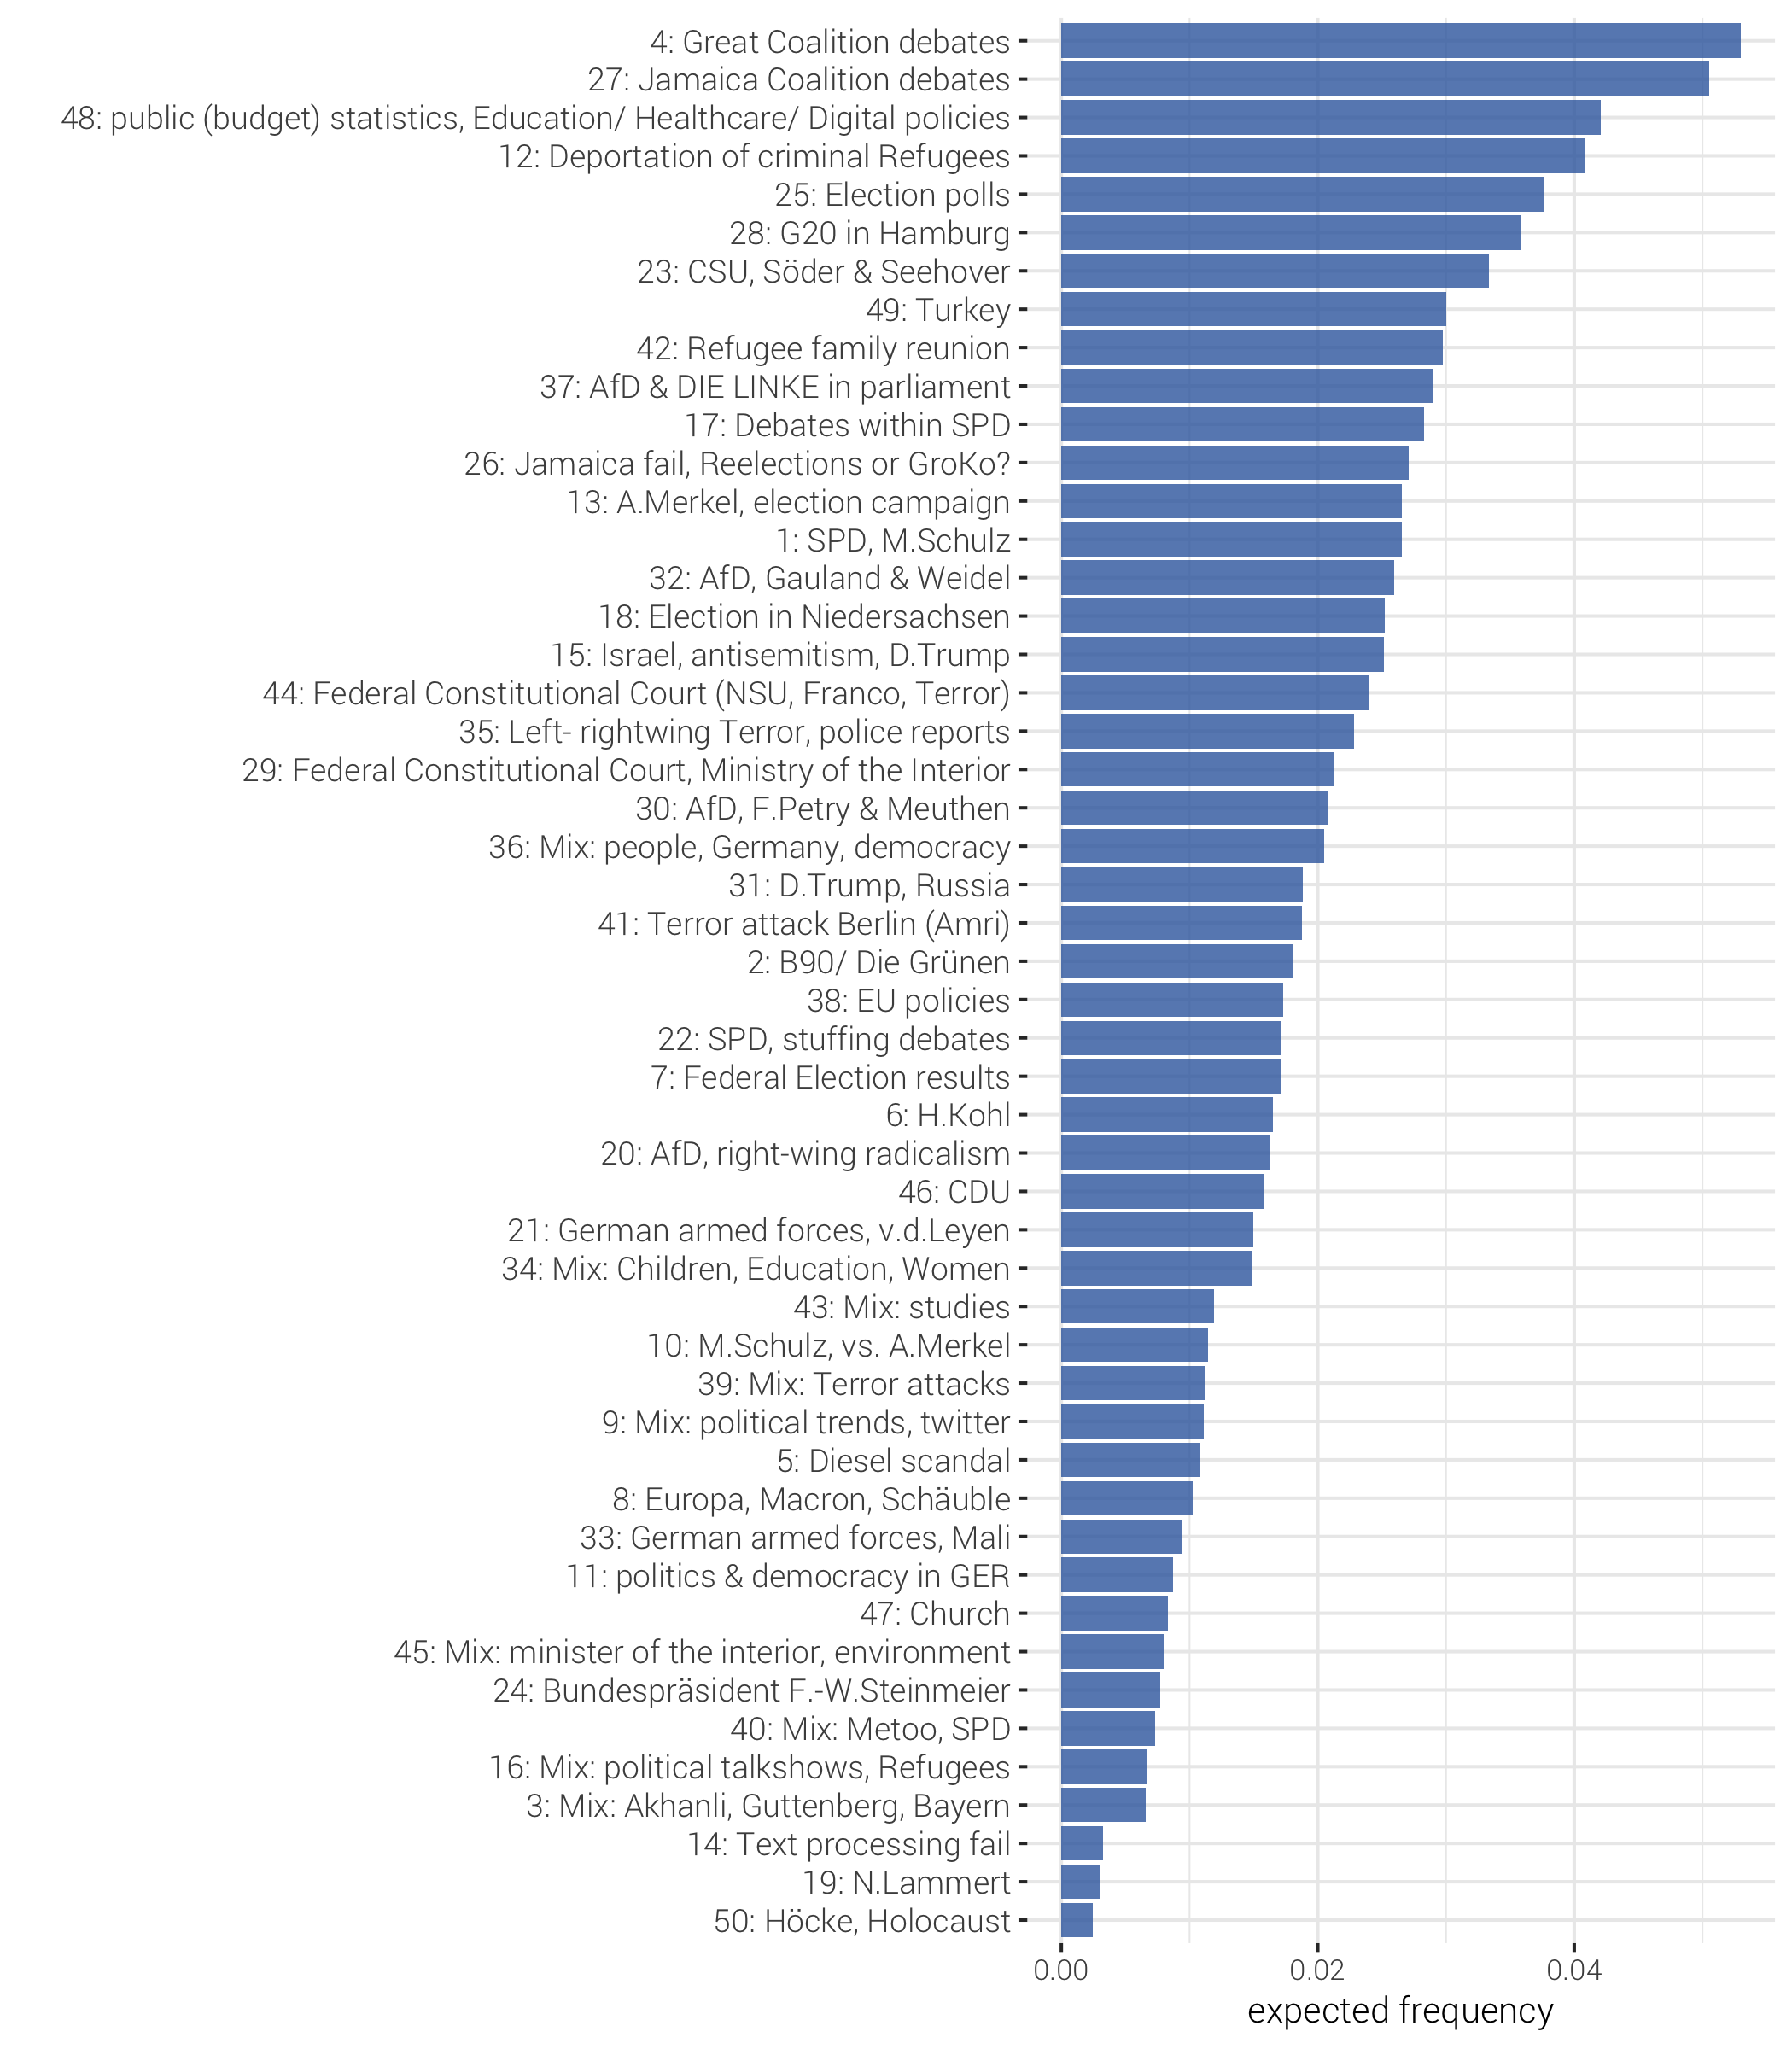
\includegraphics[width=\textwidth,keepaspectratio]{../figs/topic_proportion.png}
		\label{fig_topic_proportion}
\end{center}
\end{figure}

We will select the following topics from the whole set (topics are ordered regarding their overall corpus frequency). The most frequent words of these topics can be seen in the appendix:

\begin{enumerate}
	\item Topic 4: Covering the debates about the great coalition talks, mainly after the failure of the Jamaica coalition talks. 
	\item Topic 27: Covering the Jamaica coalition talks, mainly focusing on the smaller players Bündnis B90/Die Grünen and FDP.
	\item Topic 23: About issues regarding the CSU, mainly about the competition between Horst Seehofer and Markus Söder and the negotiations with the CDU.
	\item Topic 37: Covering debates of AfD and DIE LINKE in the parliament (Deutscher Bundestag).
	\item Topic 17: Covering votes within the SPD, mainly regarding the vote about a possible coalition with CDU/CSU ("GroKo")
	\item Topic 26: Discussing the failure of the Jamaica coalition talks and the two possible alternatives: Reelections or a great coalition.
	\item Topic 13: About Angela Merkel, mainly right before the election.
	\item Topic 1: About the SPD, mainly about the election campaign and Martin Schulz as candidate for the chancellor.
	\item Topic 32: About the AfD, mainly about Alice Weidel and Alexander Gauland, voted as parliamentary party leaders after the resignation of Frauke Petry.
	\item Topic 30: About the AfD, mainly about the resignation of Frauke Petry and Jörg Meuthen.
	\item Topic 2: About B90/Die Grünen, mainly covering issues regarding the party's personell debates.
	\item Topic 22: About SPD, mainly covering issues regarding the party's personell debates
	\item Topic 20: About the AfD, mainly about their relation to right-wing extremist groups.
	\item Topic 46: Covering issues regarding the CDU.
\end{enumerate}   

Next, the differences of topic prevalence for given document characteristics can be estimated \citep{roberts_model_2016}. More specifically, I estimate a linear model, where the documents are observations, the dependent variable is the posterior probability of a topic and the covariates are the metadata of documents (see equation \ref{eq_1}). The stm-package provides a function that uses the method of composition to incorporate uncertainty in the dependent variable, drawing a set of topic proportions from the variational posterior repeated times and compute the coefficients as the average over all results \citep{roberts_stm:_2016}.
% Letzten satz umschreiben! hört sich sonst so an als würde ich nicht wissen, was die macht. 
% Formel erklären! 

\begin{equation}\label{eq_1}
	\theta_d=\alpha+\beta x_{newswire}+\epsilon
\end{equation}

Figure \ref{fig_estimateEffects} shows the regression results for the above selected topics. The coefficients indicate the deviation from the base value of Bild.de. Starting from above it becomes apparent that the topic prevalence of topic 46 (regarding the CDU) is significantly less for Tagesschau.de and Stern.de. The other media do not show any significant difference to Bild.de for this topic. The opposite is true for topic 37: With the exception of Stern.de and DIE WELT, topic prevalence for this topic is significantly higher for all media than for Bild.de. With the following two topics on AfD it is striking that the topic prevalence at Tagesschau.de is significantly lower compared to Bild.de. The topics concerning the Jamaican coalition (topic 27) and the failure (topic 26) seem to be discussed most likely at Bild.de. The case is different for the CSU issue (Topic 23), where SPIEGEL ONLINE has the highest probability. The same applies to the topic related to the personnel debates of the SPD (22). However, Bild.de has the highest topic prevalence for the topic related to votes within the SPD, especially the vote on the grand coalition. The same applies to the topic regarding the SPD in general and Martin Schulz in particular (1). Overall, topics concerning the SPD seem to be more frequent at Bild.de than in the other media. Moreover, the distribution of topics at FOCUS ONLINE seems to be the most similar to that of Bild.de, while the biggest differences exist between Bild.de and Tagesschau.de. 

\begin{figure}[H]
	\caption{Regression results}
		\begin{center}
			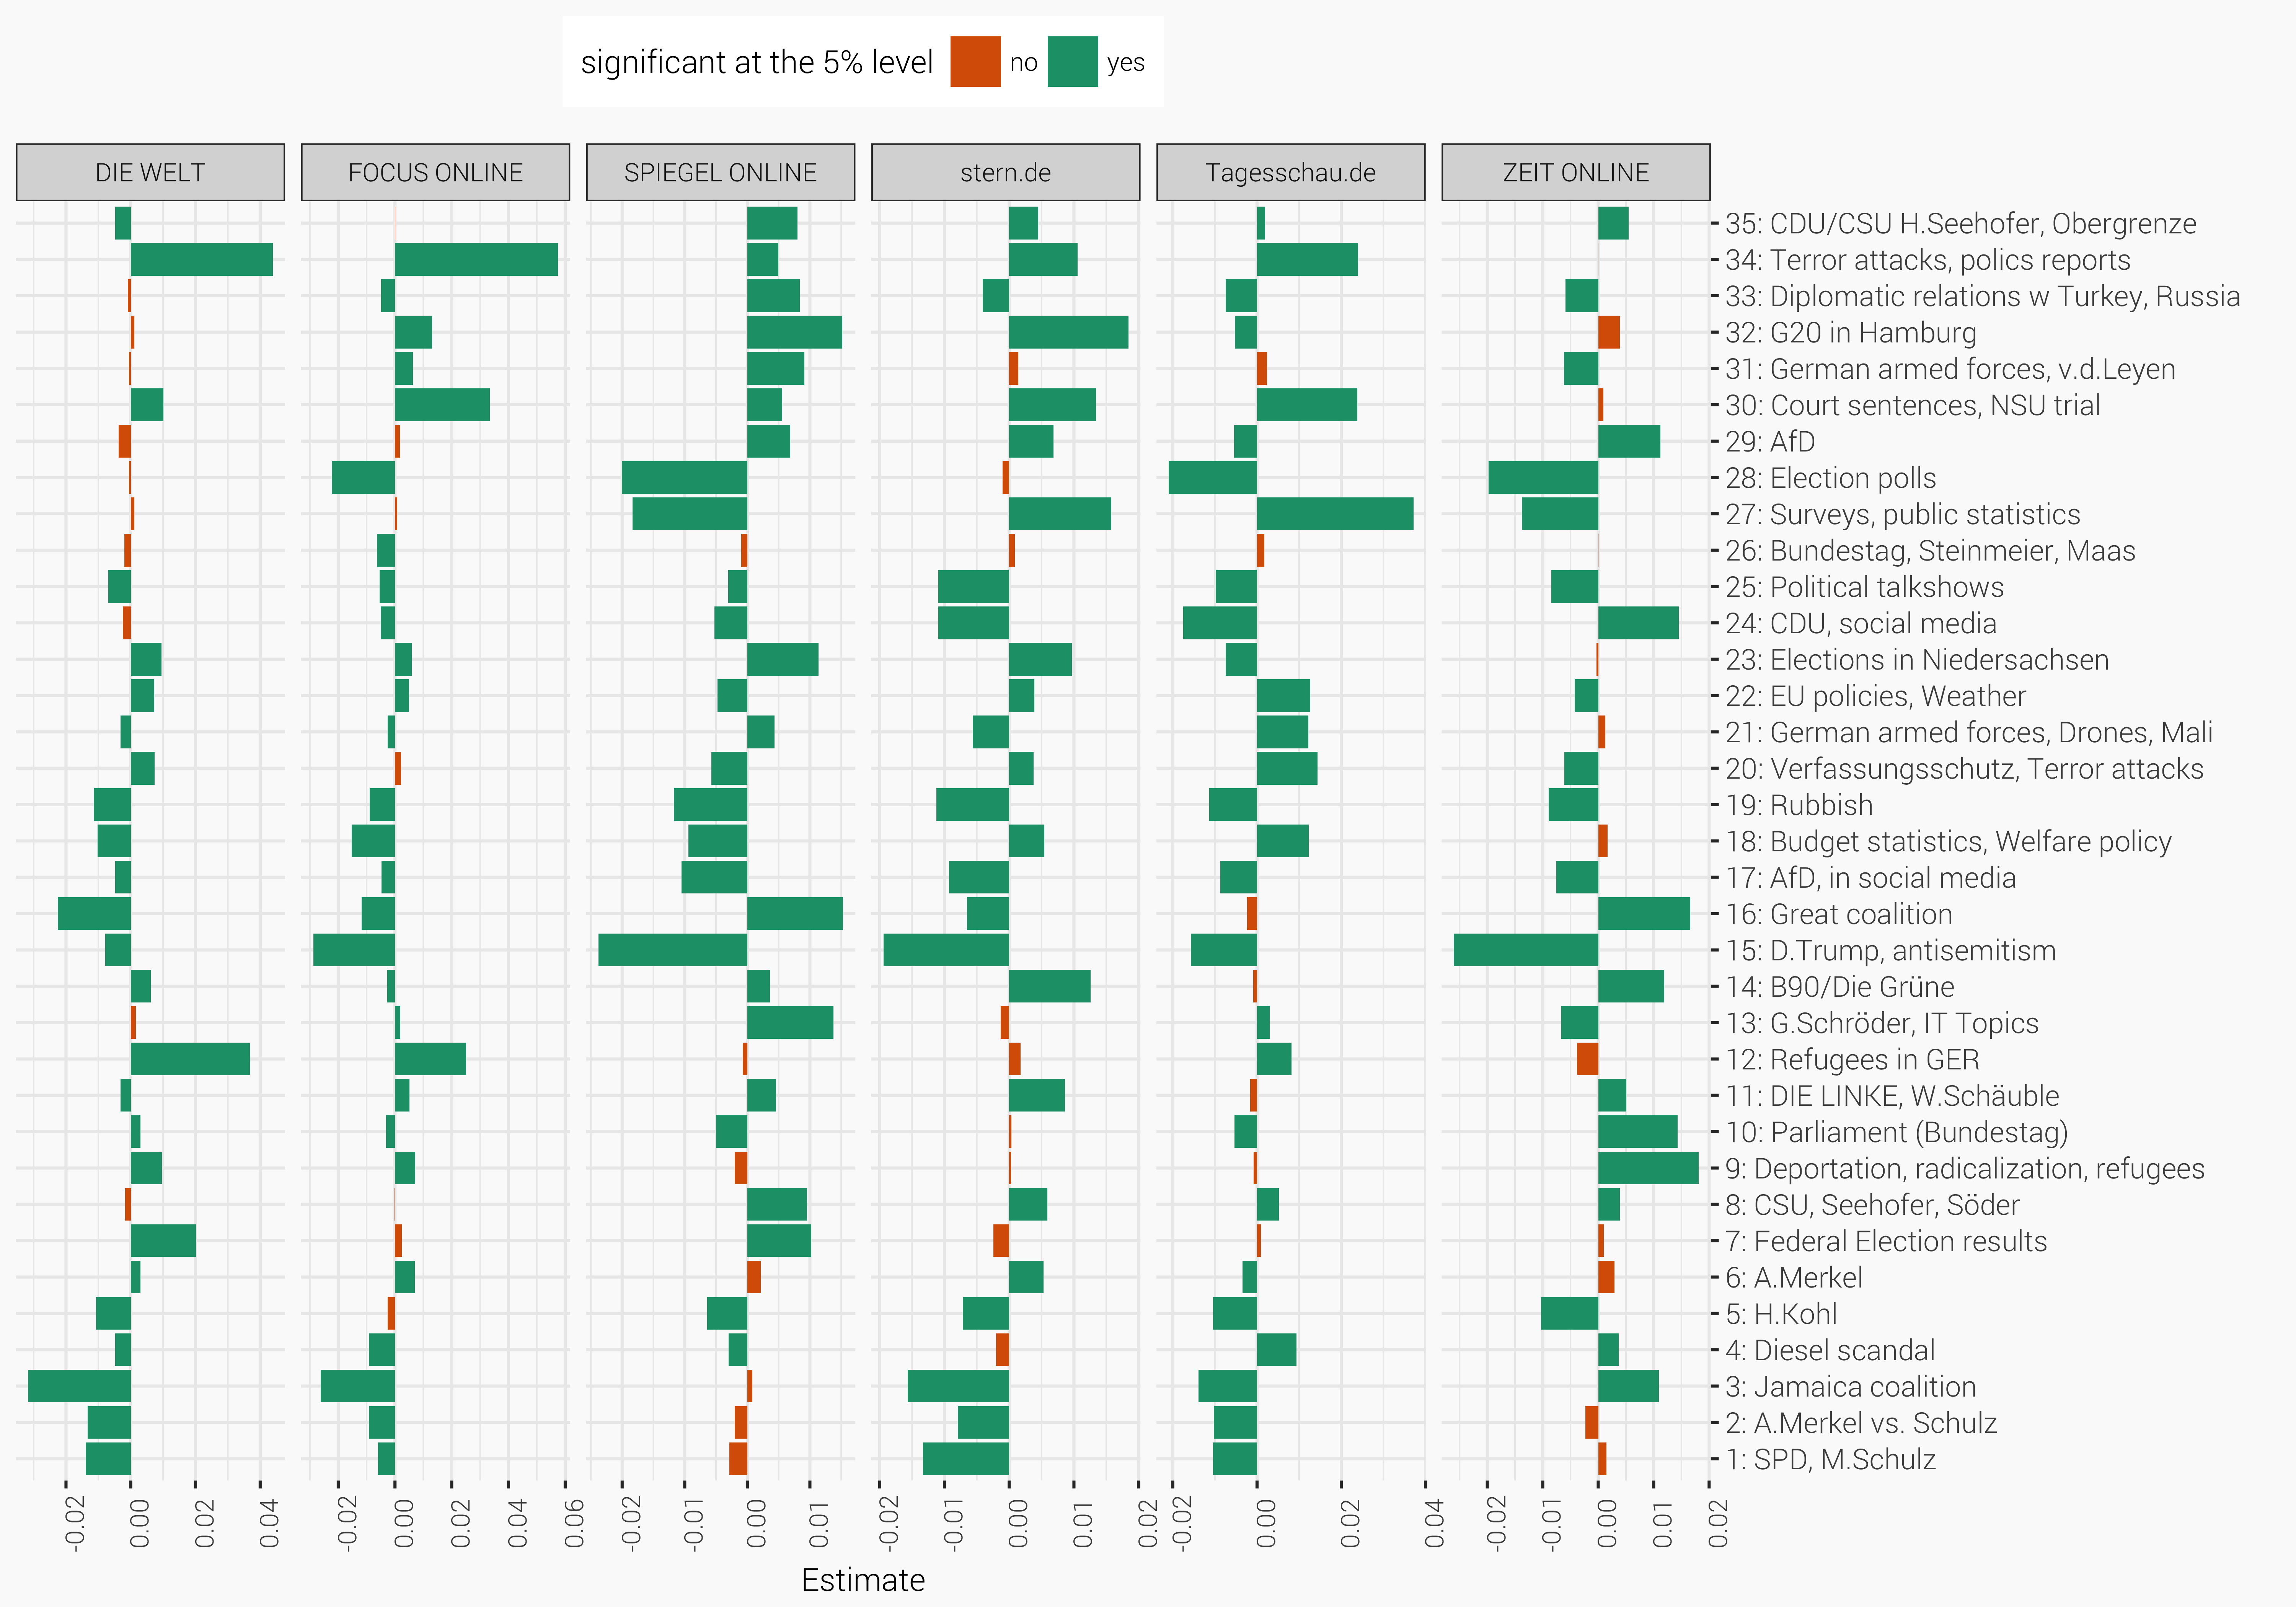
\includegraphics[width=\textwidth,keepaspectratio]{../figs/estimates.png}
		\end{center}
	\label{fig_estimateEffects}
\end{figure}

\subsection{Tone}\label{subsection_tone}

The sentiment analysis is conducted with those documents that are assigned to one of the above selected topics with the highest probability. A dictionary-based method is then applied on the remaining 5611 documents with the aim to measure the tone (or sentiment) of a document. The idea of a sentiment analysis is to determine the attitude of a writer toward the overall tonality of a document. To conduct such an analysis, a lists of words (dictionary) associated with a given emotion, such as negativity is pre-defined by the analyst. The document is then deconstructed into individual words and the frequencies of words contained in a given dictionary are then calculated. 

Such lexical or “bag-of-words” approaches are widely presented in the finance literature to  determine  the  effect  of  central  banks’  monetary  policy  communications on asset prices and real variables (\citet{nyman_news_2018} \citep{tetlock_giving_2007}, \citep{tetlock_more_2008}). \citet{hansen_shocking_2016} use a similar approach to measure "the two Ts" (Topic and tone). They explore the effects of FOMC (Federal Open Market Committee) statements on both market and real economic variables. To understand the multi-dimensional information a statement is transmitting, they apply LDA on a corpus of 142 FOMC decision statements split into sentences (topic). They then measure how the central bank is talking about that topic, using a dictionary approach (tone). To calculate their score, they subtract the negative words from the positive words und divide this by the number of total words of the statement. A similar score is used by \citet{nyman_news_2018}, who measure the effect of narratives and sentiment of financial market text-based data on developments in the financial system. They count the number of occurrences of excitement words and anxiety words and then scale these numbers by the total text size as measured by the number of characters.

The present paper uses a dictionary that lists words associated with positive and negative polarity weighted within the interval of $[-1; 1]$. SentimentWortschatz\footnote{SentiWS for short. available here: http://wortschatz.uni-leipzig.de/de/download}, is a publicly available German-language resource for sentiment analysis, opinion mining etc. The current version of SentiWS (v1.8b) contains 1,650 positive and 1,818 negative words, which sum up to 15,649 positive and 15,632 negative word forms incl. their inflections, respectively. The sentiment score for each document $d$ is calculated  based on the weighted polarity values for a word, defined on an interval between -1 and 1. The score is then calculated from the sum of the words in a document (which can be assigned to a word from the dictionary) divided by the total number of words in that document:
 
\begin{equation}
	\text{SentScore}_d = \frac{|\text{positive polarity score}_d| - |\text{negative polarity score}_d|}{|\text{TotalWords}_d|}
\end{equation}

The following figure shows the results of the analysis for each topic on a monthly basis, aggregated on all newspaper. Each sentiment value is weighted by the relative share of the topic in the overall reporting of that month.

Some conclusions can be drawn from this illustration. First of all, it can be seen that, on average, all topics are discussed almost exclusively negatively. An exception is topic 27 concerning the Jamaica coalition negotiations, which shows a positive sentiment value for a short period of time (October 2017). In the following month (November 2017), after it became clear that there would be no coalition between the CDU/CSU, FDP and Die Grünen, the value of this topic as well as that of topic 26 drops rapidly, but then rises again in February. Concerning the issues that discuss the great coalition between CDU/CSU and SPD, it is evident that the overall tone is in which this topic is discussed is generally decreasing from November 2017 to January 2018, but in the following February, the sentiment value of this topic rises. However, the sentiment score of topics that deal with the SPD (1, 17, 22) is diminishing in the course of time, with topic 17 recording the largest decline. For the other parties the process is rather zigzag-like.

\begin{figure}[H]
	\caption{Monthly Sentiment Score}
		\begin{center}
			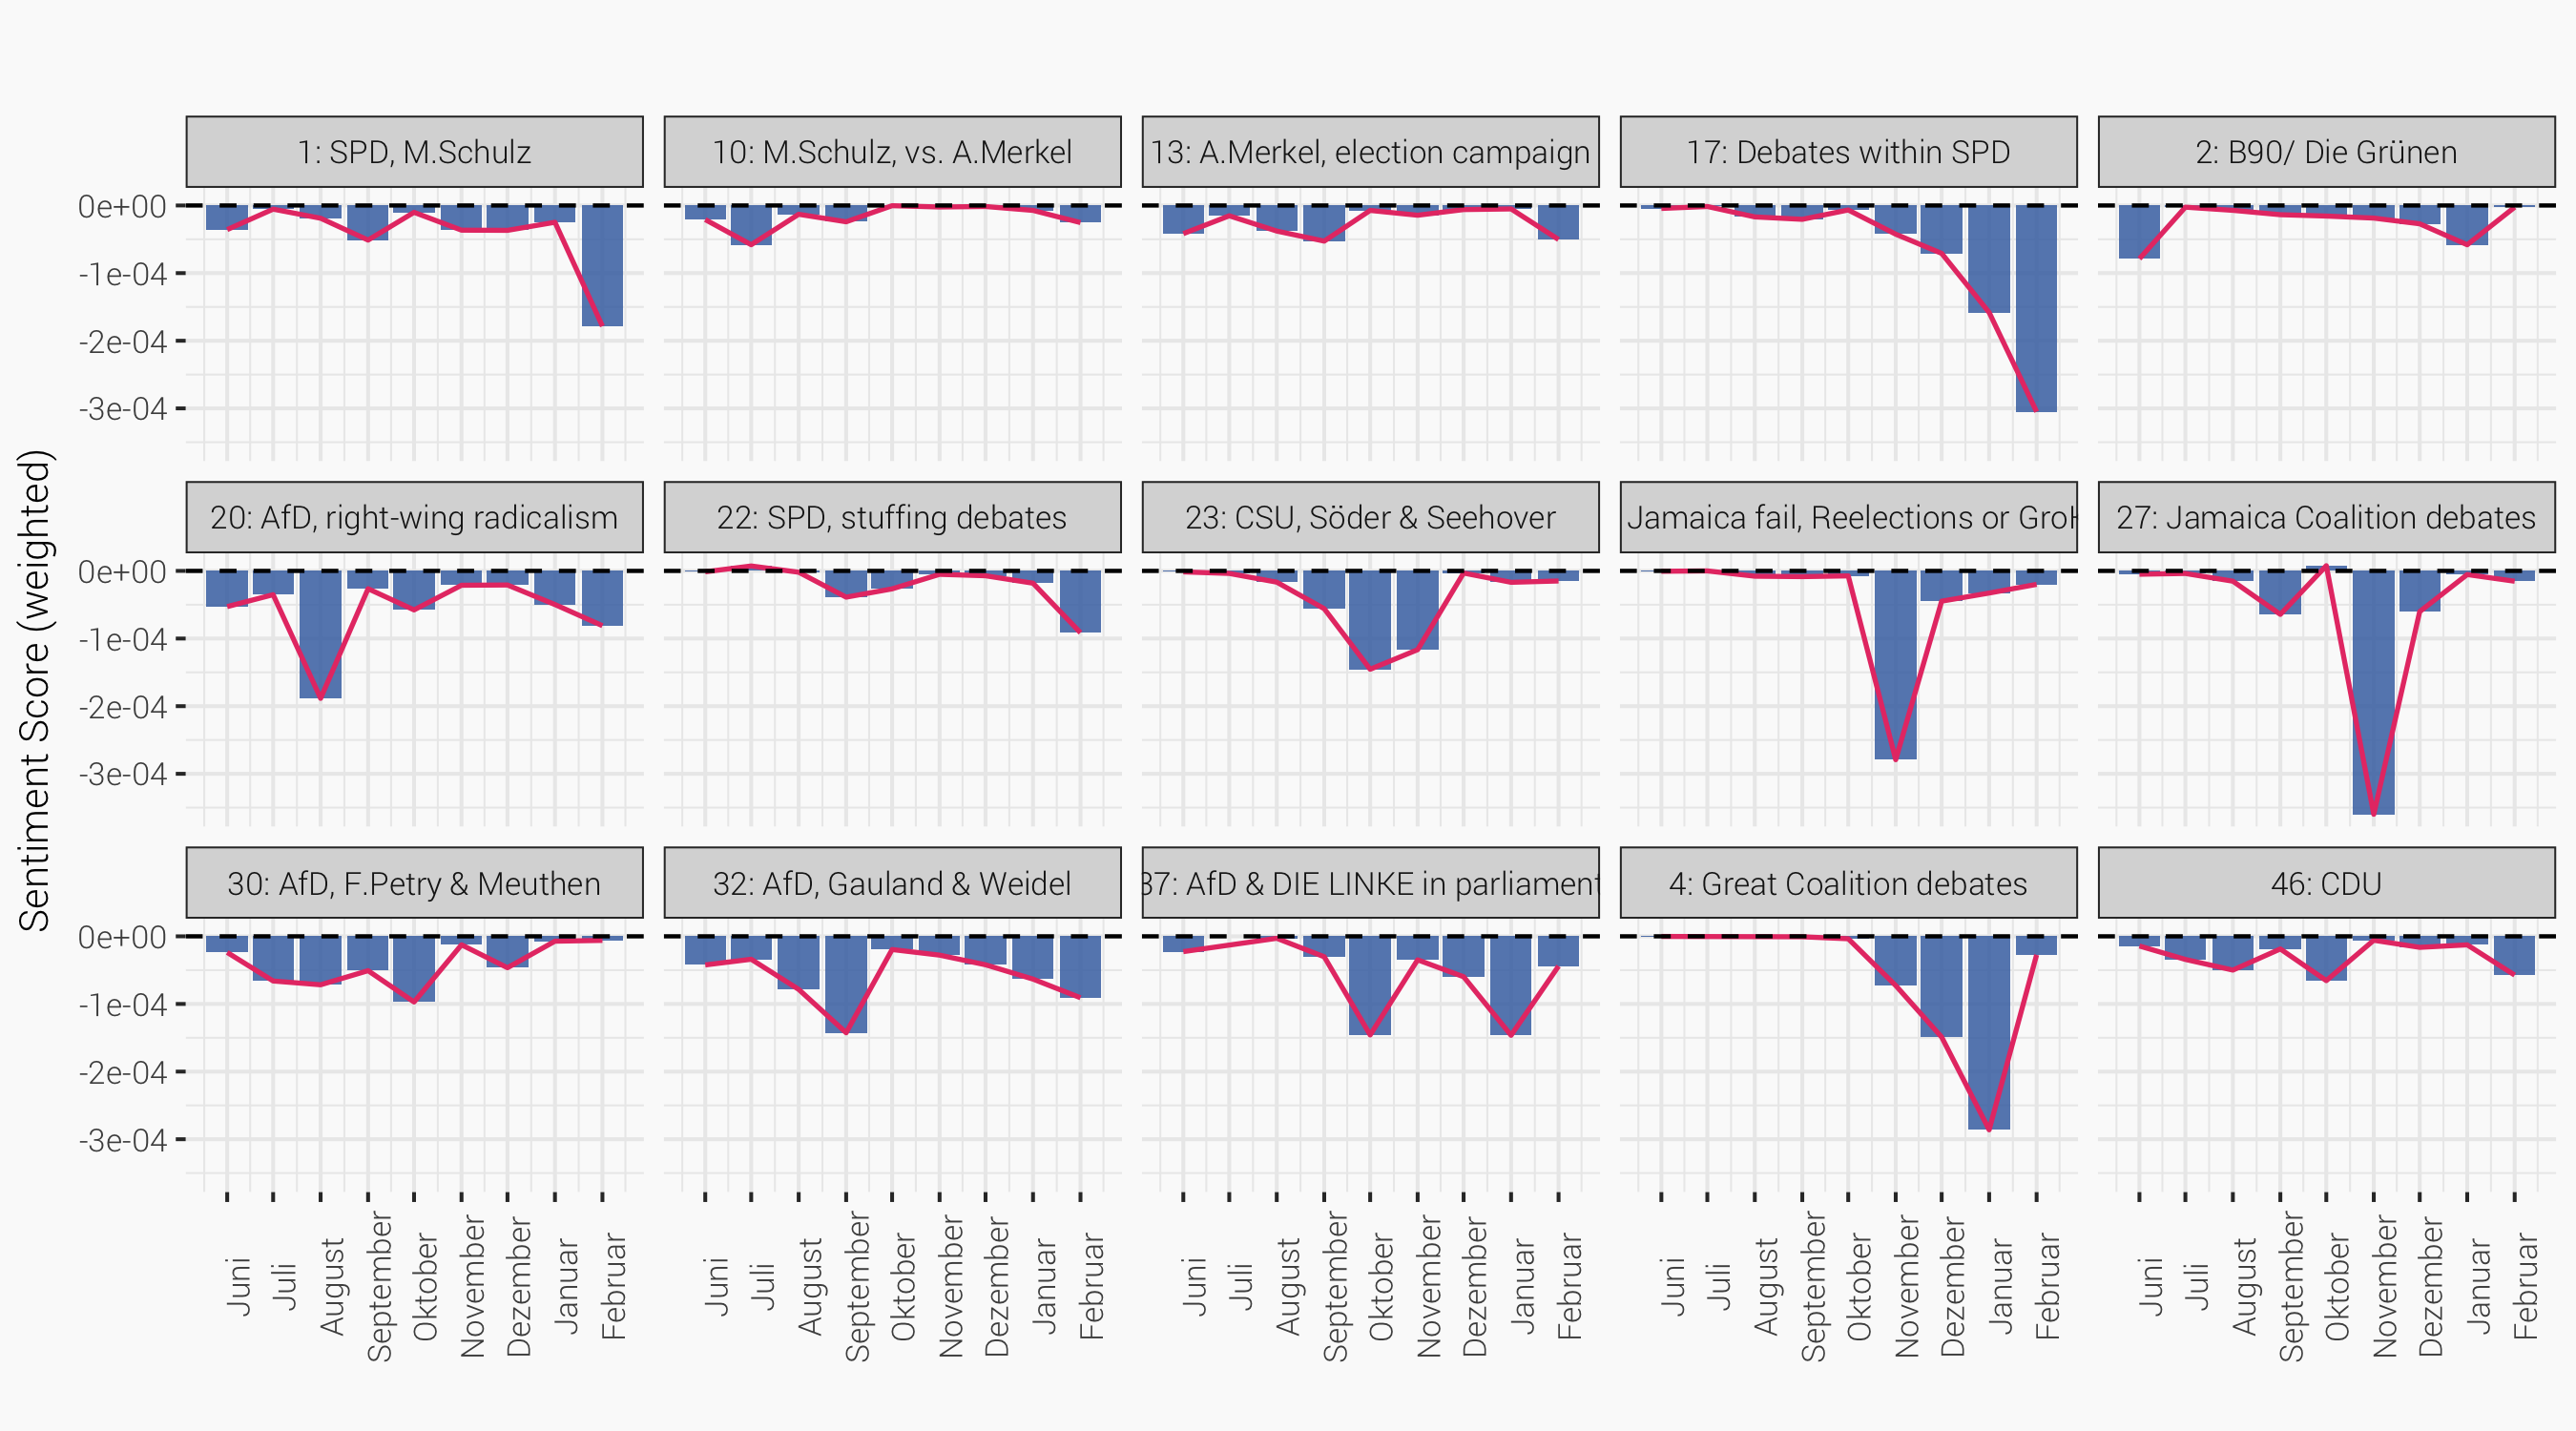
\includegraphics[width=\textwidth,keepaspectratio]{../figs/sentscore_monthly.png}
		\end{center}
	\label{fig_sentscore_monthly}
\end{figure}

If aggregated by news provider, some differences between the sites are discernible (Figure \ref{fig_sentscore_site}\footnote{The numbers reflect the number of observations.}). To begin with, it can be noted that on average all topics are discussed negatively by all news providers, except topic 22, which mainly covers the personnel debates of the SPD and has a positive value at Tagesschau.de. One striking feature is the way in which the Jamaica negotiations and their failure are reported (topics 27 and 26). Although all providers discuss this topics in a negative light, Bild.de reports them particularly negative. The same applies to the reports on the grand coalition, where the value of ZEIT ONLINE is the most negative. 

We use two different Figures to analyze the differences between the media outlets graphically: We use the bar plot to examine the polarity tendencies of the individual topics within a medium (\ref{fig_sentscore_site}) and the radar plot to observe the differences between the media (\ref{fig_sentscore_radar}).

Starting with the bar plot it becomes apparent that all topics are discussed negatively, except topic 23 at Tagesschau.de. At Bild.de, the topics that include the coalition negotiations (26,27,4) and the SPD (1,17) are the most negative. The topics relating to AfD (20,30,32,37) are also discussed more negatively. Looking at the values of WELT ONLINE, two of the AfD topics have the most negative value (32.20). Topic 27 concerning the Jamaica Coalition (27) and the Grand Coalition (4) also score relatively negatively. Concerning FOCUS ONLINE, it is mainly topics that relate to the SPD (27, 17, 4, 1) that have a strong negative sentiment value, together with topic 32 and 37. Turning to SPIEGEL ONLINE, it is noticeable that the difference in sentiment value between the individual topics is less pronounced. Topics 13 and 10 stand out as comparatively less negative. However, these issues are also the least negatively discussed in the other media. Also at stern.de the difference in sentiment value is less significant and overall less negative. The topics regarding CDU (46) and Martin Schulz (10) score the most positively (or least negatively). Tagesschau.de is the least negative on most topics, or even once positive. However, this does not apply to topic 23 (CSU), where tagesschau.de is most negative in comparison to the other media. As with Bild.de, the issues relating to the coalition negotiations (27 and 4) also come off rather badly with ZEIT ONLINE. However, the issues surrounding AfD (30, 32, 37 and 20) are even more negative than at Bild.de. 

\begin{figure}[H]
	\caption{Sentiment Score by news wire}
	\begin{center}
			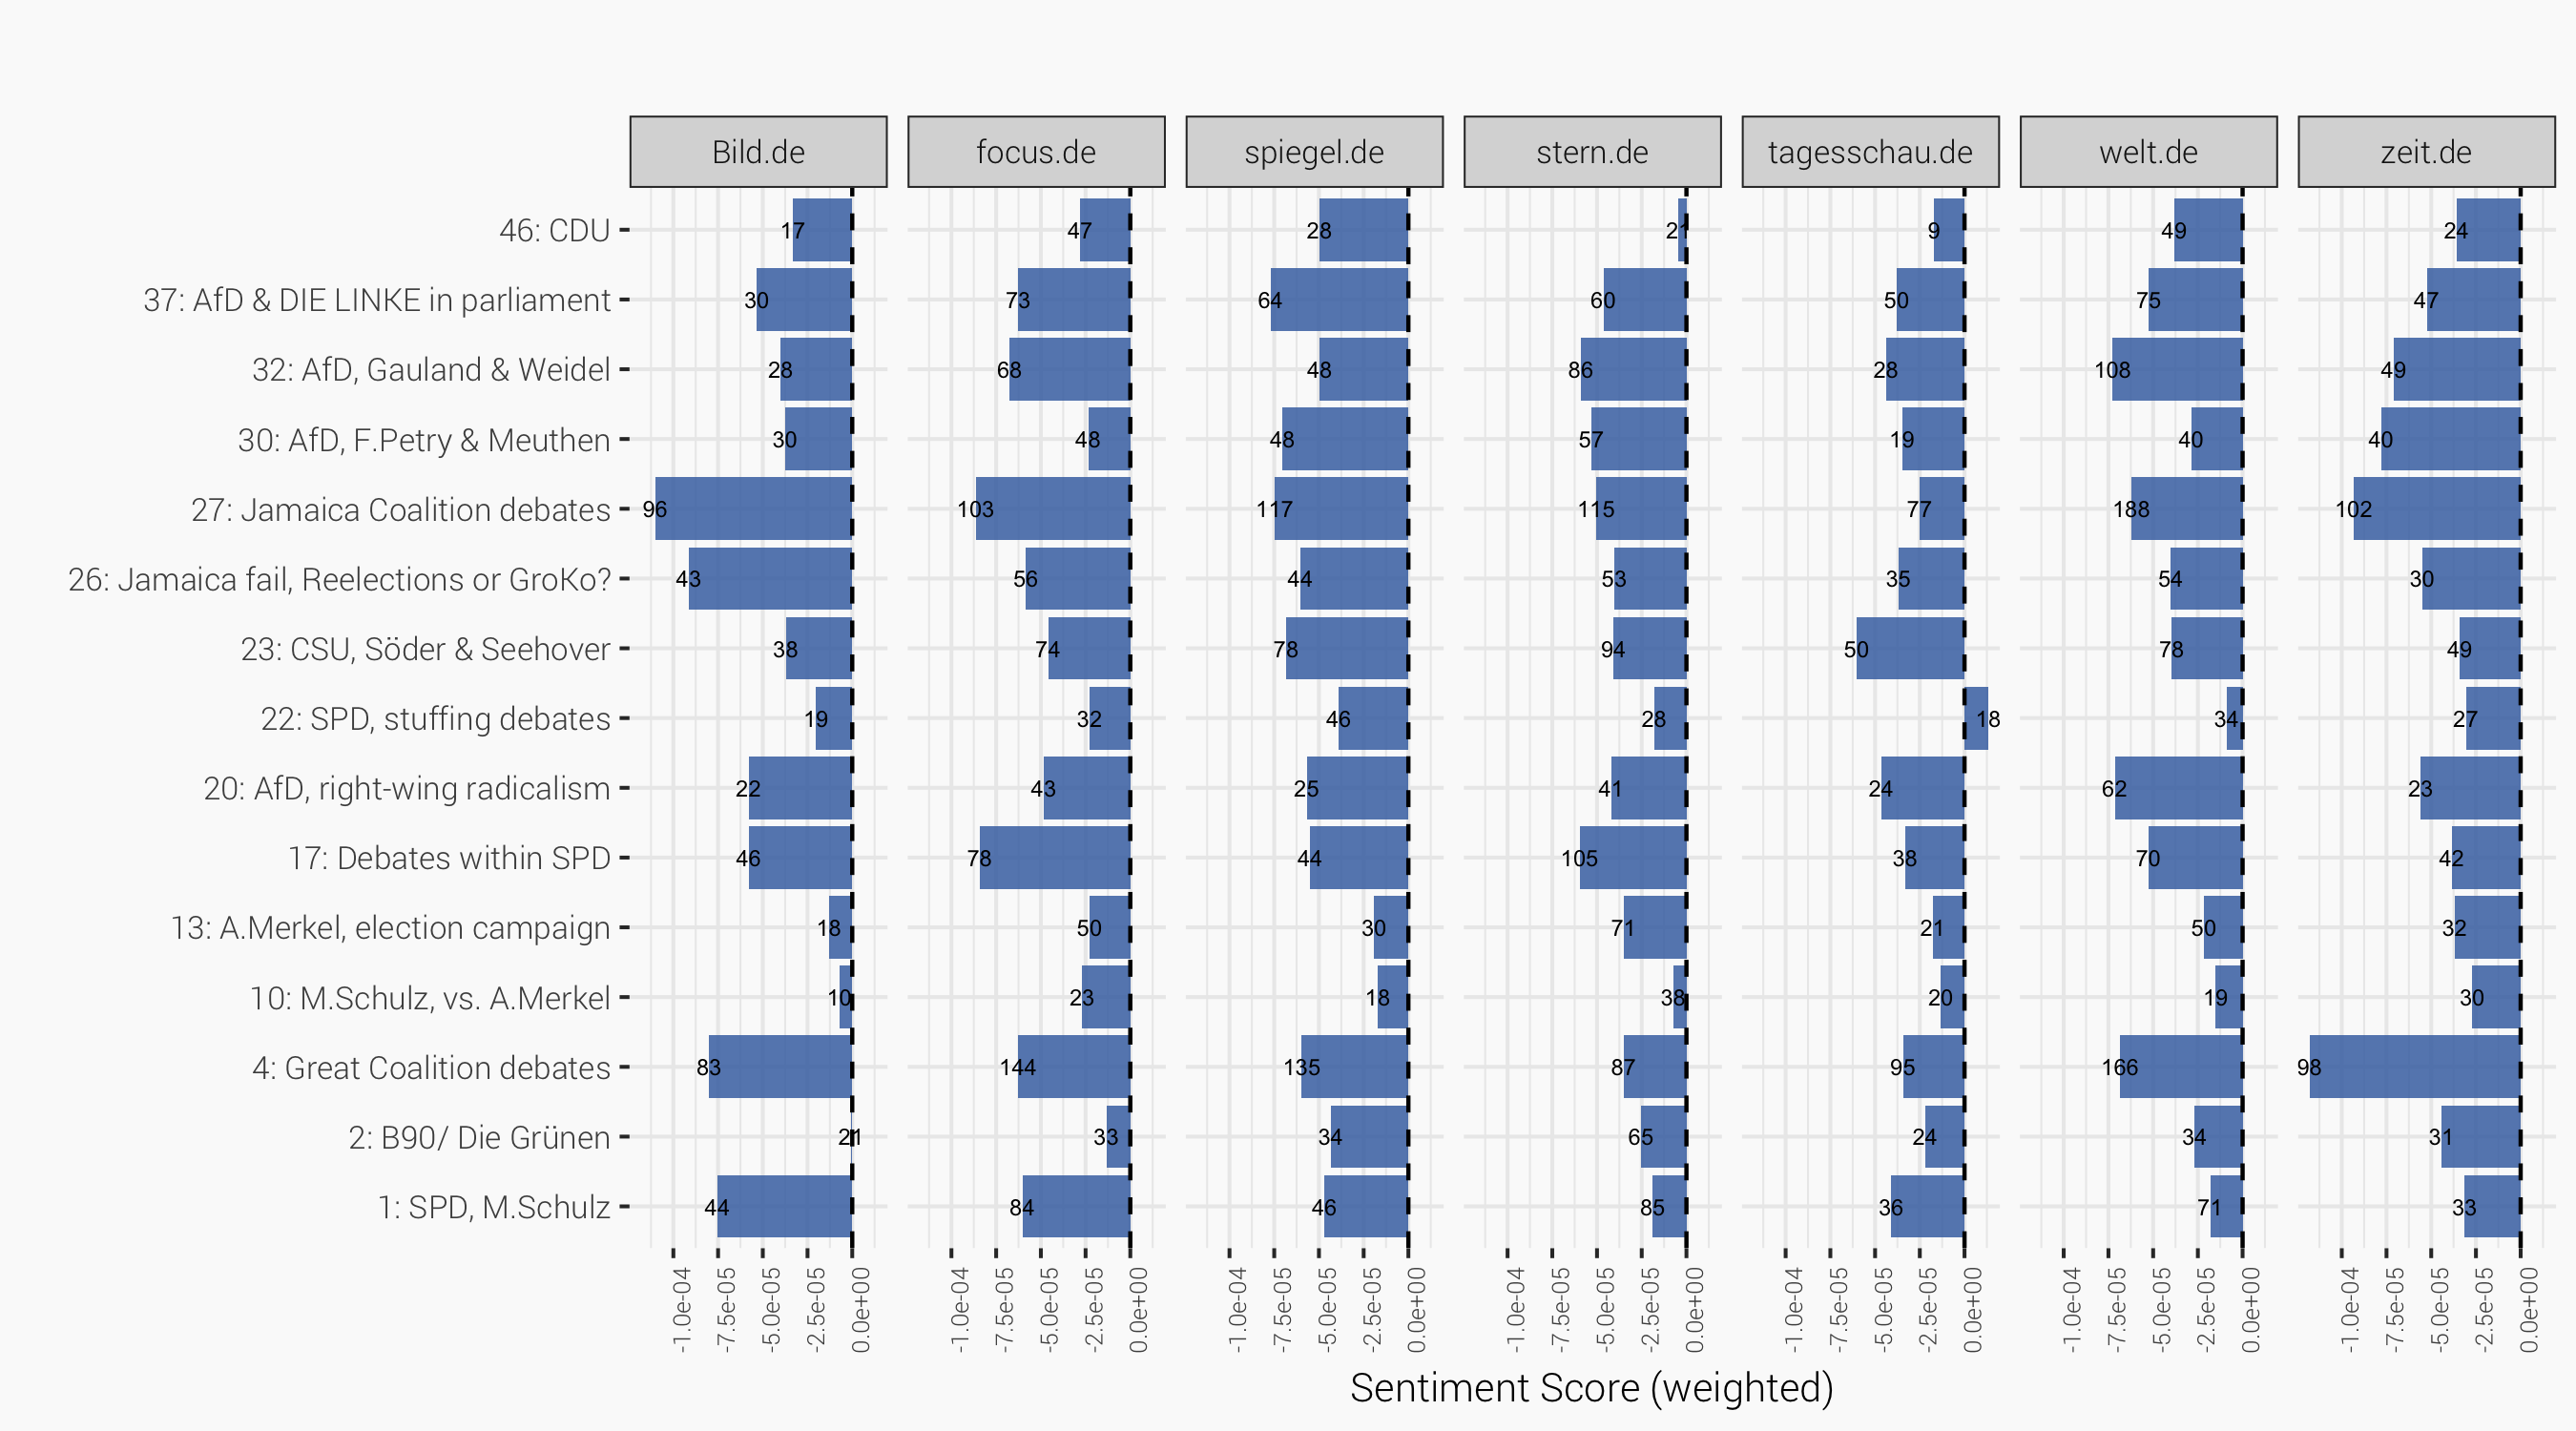
\includegraphics[width=\textwidth,keepaspectratio]{../figs/sentscore_site.png}
			\label{fig_sentscore_site}
	\end{center}
\end{figure}

A good overview of how differently the topics are discussed by the providers is shown in Figure \ref{fig_sentscore_radar}. It gets evident that the sentiment value of the media differs most notably with regard to topic 27 and topic 4, i. e. the topics on which the coalition negotiations are reported. With regard to the Jamaica coalition, Bild.de reports the most and tagesschau.de the least negative. The reporting of ZEIT ONLINE concerning the grand coalition is the one with the most negative sentiment value and again Tagesschau.de, together with stern.de, the one with the value which is least negative. Furthermore, it becomes evident that the negative sentiment value of FOCUS ONLINE regarding topic 17 is high in relation to the other media. FOCUS ONLINE thus reports comparatively more negatively on the debates within the SPD. This includes in particular the vote on a possible coalition with CDU/CSU. For topic 1, which also deals with the SPD, the value of FOCUS ONLINE is rather negative, only undercut by Bild.de. Topics related to AfD do not show striking differences. 

\begin{figure}[H]
	\caption{Sentiment Score by news wire}
	\begin{center}
			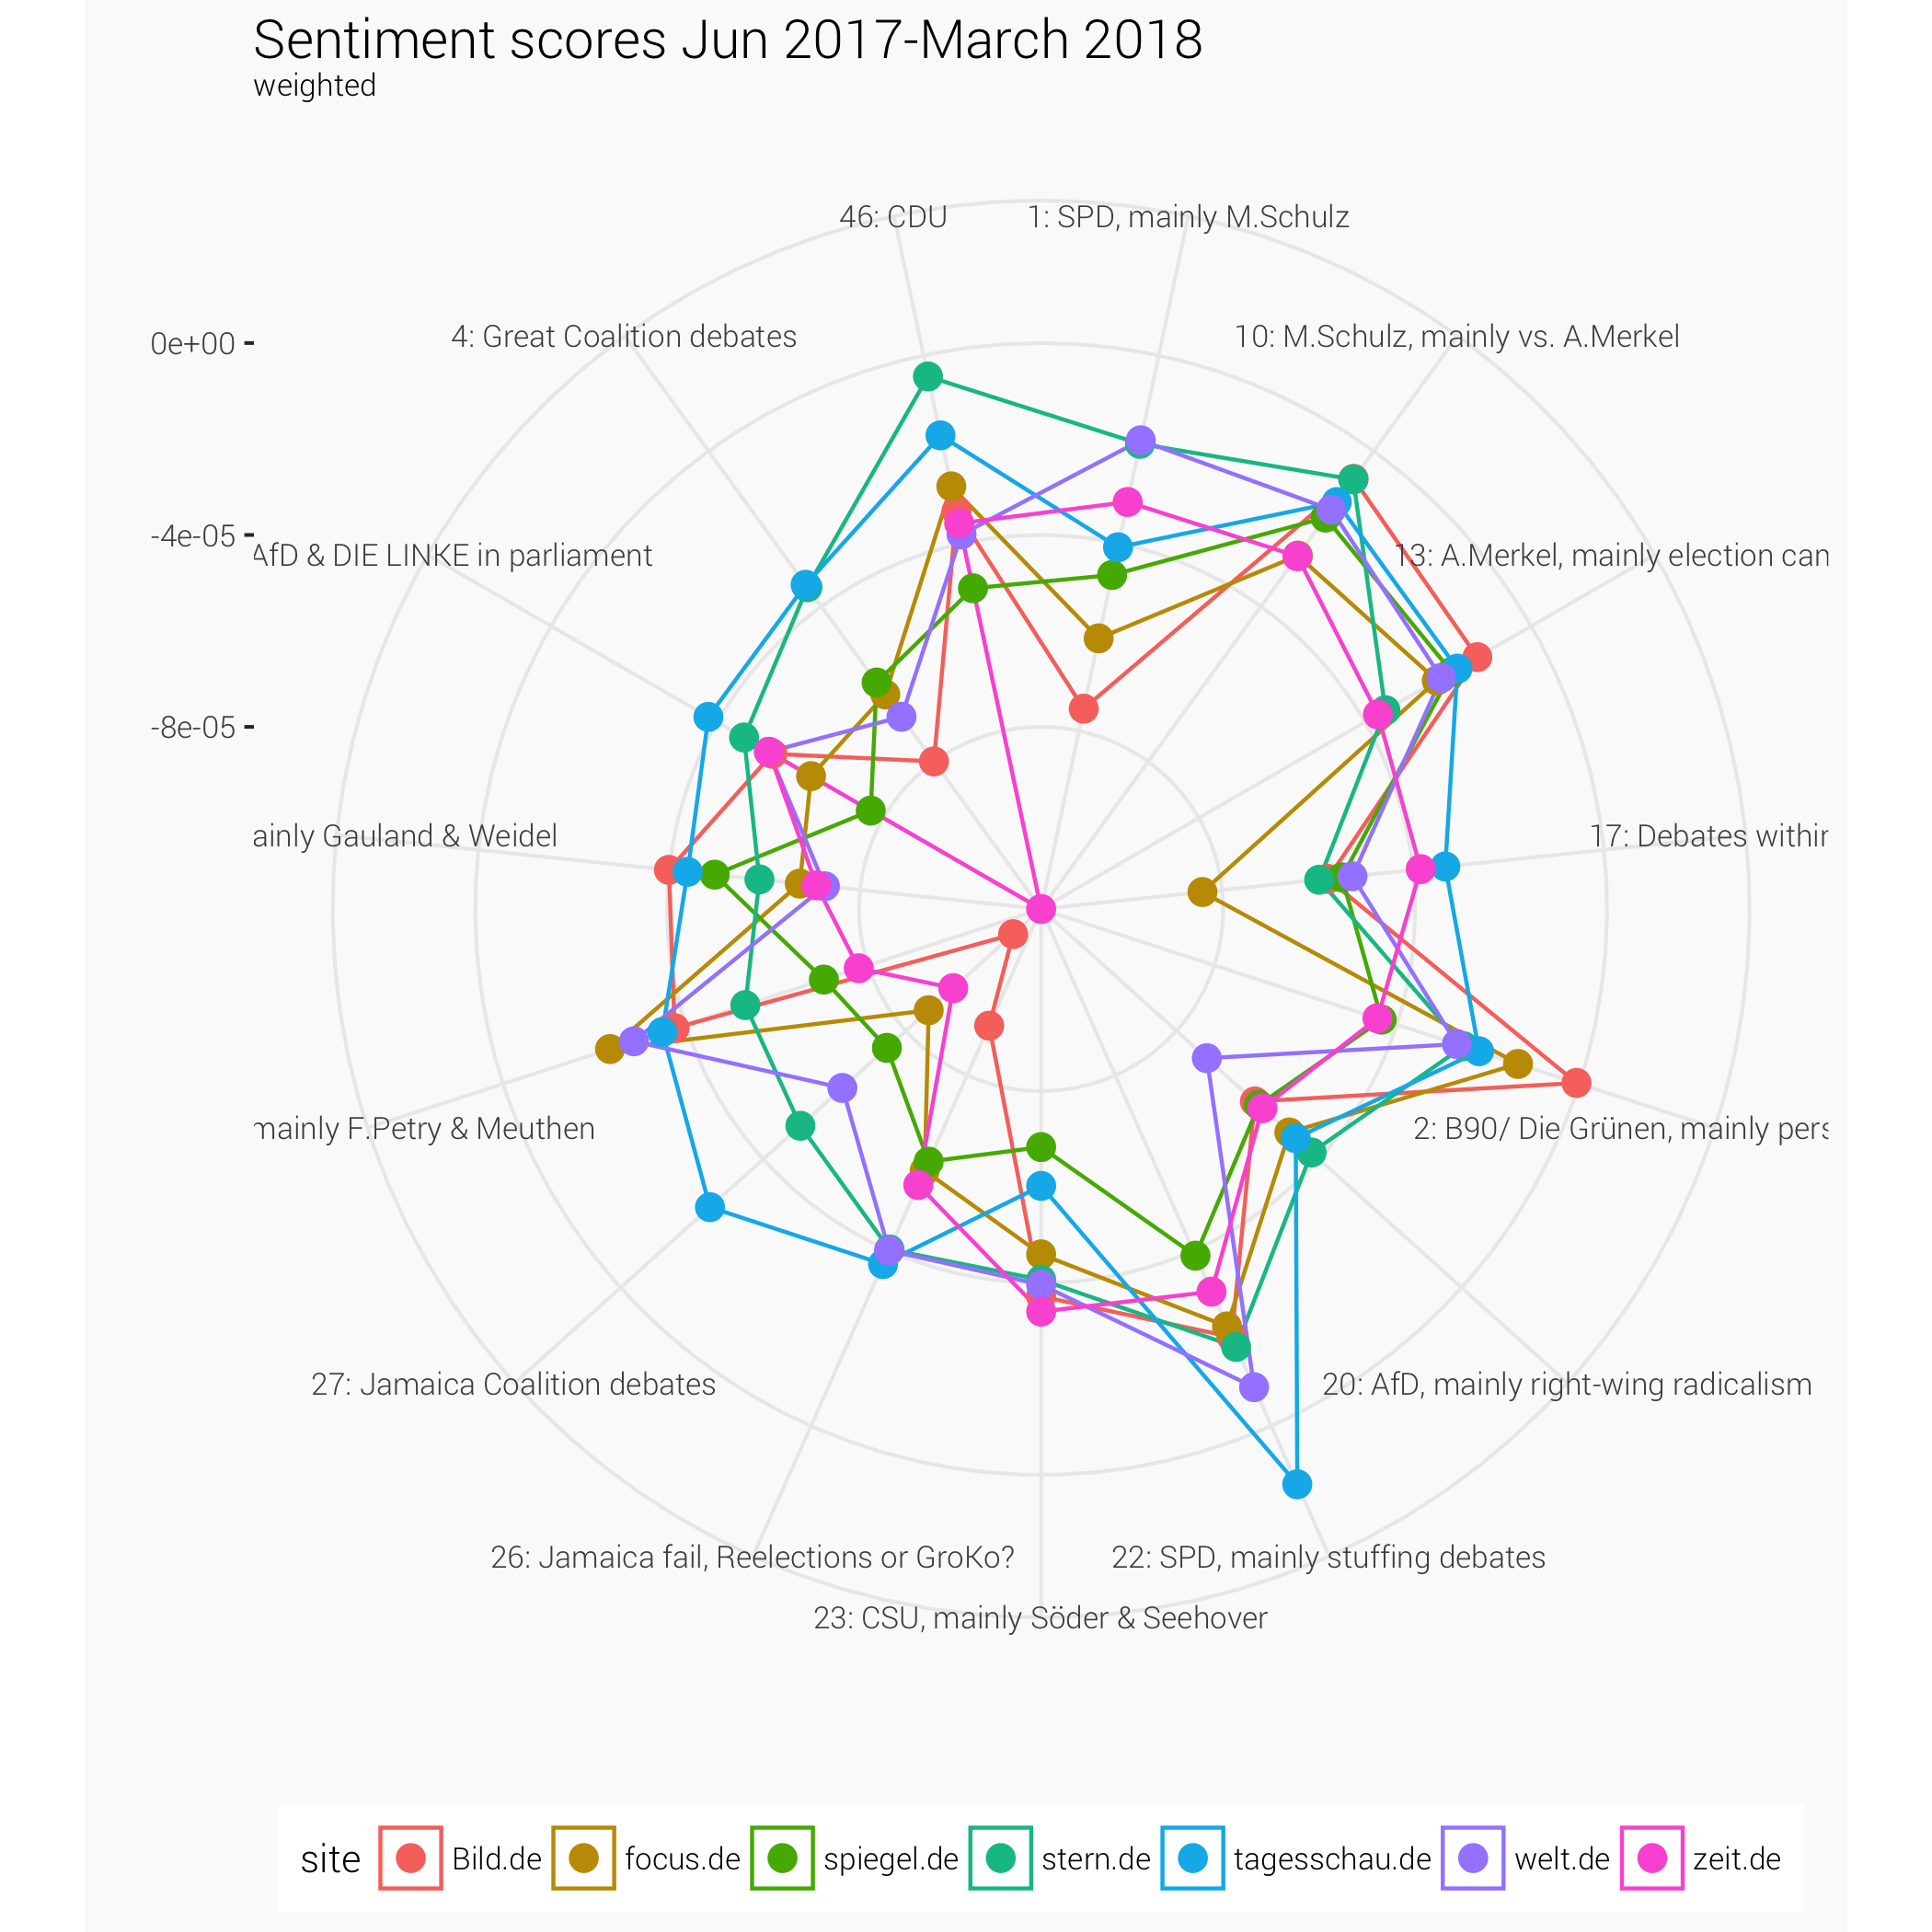
\includegraphics[width=0.8\textwidth,keepaspectratio]{../figs/sentscore_radar.png}
			\label{fig_sentscore_radar}
	\end{center}
\end{figure}

After the above figures have been analyzed, the following points can be summarized: (a) The sentiment value of the SPD is decreasing over time, especially in regard to internal votes. (b) The topics relating to the coalition talks on Jamaica (26, 27) and the grand coalition (4) are discussed rather critically, but they also show the greatest differences within the media. In contrast, the tonality of the topics in relation to the AfD shows rather small differences. (c) Overall, the sentiment value at Tagesschau.de is the least negative and only shows a comparatively strong negative value at topic 23, concerning the CSU. 

\subsection{News sentiment and poll data}\label{ch_correlation}

This section seeks to examine the temporal association between sentiment reflected in online news content and phone survey poll results in Germany. Specifically, it aims to find the extent to which online sentiment and phone survey results correlate. I use the data from the "Sonntagsumfrage" (Sunday survey) from infratest dimap\footnote{https://www.infratest-dimap.de/umfragen-analysen/bundesweit/sonntagsfrage/}. The institution regularly asks at least 1000 German citizens the question: "Which party would you choose if federal elections take place next Sunday?" The survey thus measures the current election tendencies and therefore reflects an intermediate state in the opinion-forming process of the electoral population.

Much of the research on online content and political trends have focused on traditional weblogs and social media websites, such as Twitter, Facebook, MySpace, and YouTube. These studies have shown that social media is used to spread political opinions and that these considerations reflect the political landscape of the offline world. \citet{tumasjan_predicting_2010} investigate Tweets between August 13th and September 19th, 2009, prior to the German national elections to examine whether Twitter messages reflect the current offline political sentiment and whether it can be used to predict the popularity of parties or coalitions in the real world. With regard to the later question, they compare the share of attention the political parties receive on Twitter with the election result to examine whether the activity on Twitter can serve as a predictor of the election outcome. They found that the number of tweets reflects the election result and even comes close to traditional election polls.

\citet{fu_analyzing_2013} use a corpus of online posts from discussion forums and blogs to examine the extent to which online sentiment reflected in social media content can predict phone survey results in Hong Kong. They build a sentiment classifier conducting a support vector machine analysis on a training set of 2,000 manually labeled posts. In order to evaluate the temporal relationship between the time series of the online sentiment score and the results of the telephone survey, a cross correlation analysis was conducted, using the Box and Jenkins autoregressive integrated moving average (ARIMA) method \citep{box_time_2008}. Estimating the cross-correlation functions of the residuals, they find that online sentiment scores can lead phone survey results by about 8–15 days. 

In a more recent conference paper, \citet{padmaja_evaluating_2014} identify the scope of negation in news articles for two political parties in India (BJP and UPA) to analyze how the choice of certain words used in these texts influence the sentiments of public in polls. Comparing three different sentiment analysis methods (two machine learning and one dictionary method), they observe that the choice of certain words used in political text was influencing the Sentiments in favor of BJP. They conclude that this sentiment bias might be one of the causes for the election results in 2014.

In the present paper, the comparison between monthly average of both the sentiment value of individual topics and the survey value of the parties is calculated using the cross-correlation function. It is important to notice, that the results from this analysis will give an indication whether correlation between the two time series exist, but it does not give any evidence about the causal relationship. None of the following interpretation of the cross-correlation coefficients is intended to describe a causal relationship.

Based on the contemporary coefficients of the cross-correlation estimation shown in Figure \ref{fig_ccf}, the most noticeable topics for each party are evaluated below. The AfD's survey results correlate negatively with topics relating to the SPD. The strongest positive correlation with regard to AfD-related topics can be found for topic 30. Since there are no isolated topics about the FDP, the issues surrounding the Jamaica negotiations are examined, which show a negative correlation. It is also striking that the poll results of the FDP correlate strongly negatively with the CSU topic (23). With regard to B90/Die Grünen, there is also a negative correlation to the Jamaica topics, however, it is slightly above the correlation-coefficient of the FDP. It is striking that there seems to be a strong negative correlation between the SPD issues and the poll results of the Left Party. Conversely, the survey results of the SPD correlate very positively with the SPD topics. The CDU's survey results correlate most positively with topics relating to coalition negotiations.

\begin{figure}[H]
	\caption{Cross-Correlation at lag 0}
	\begin{center}
			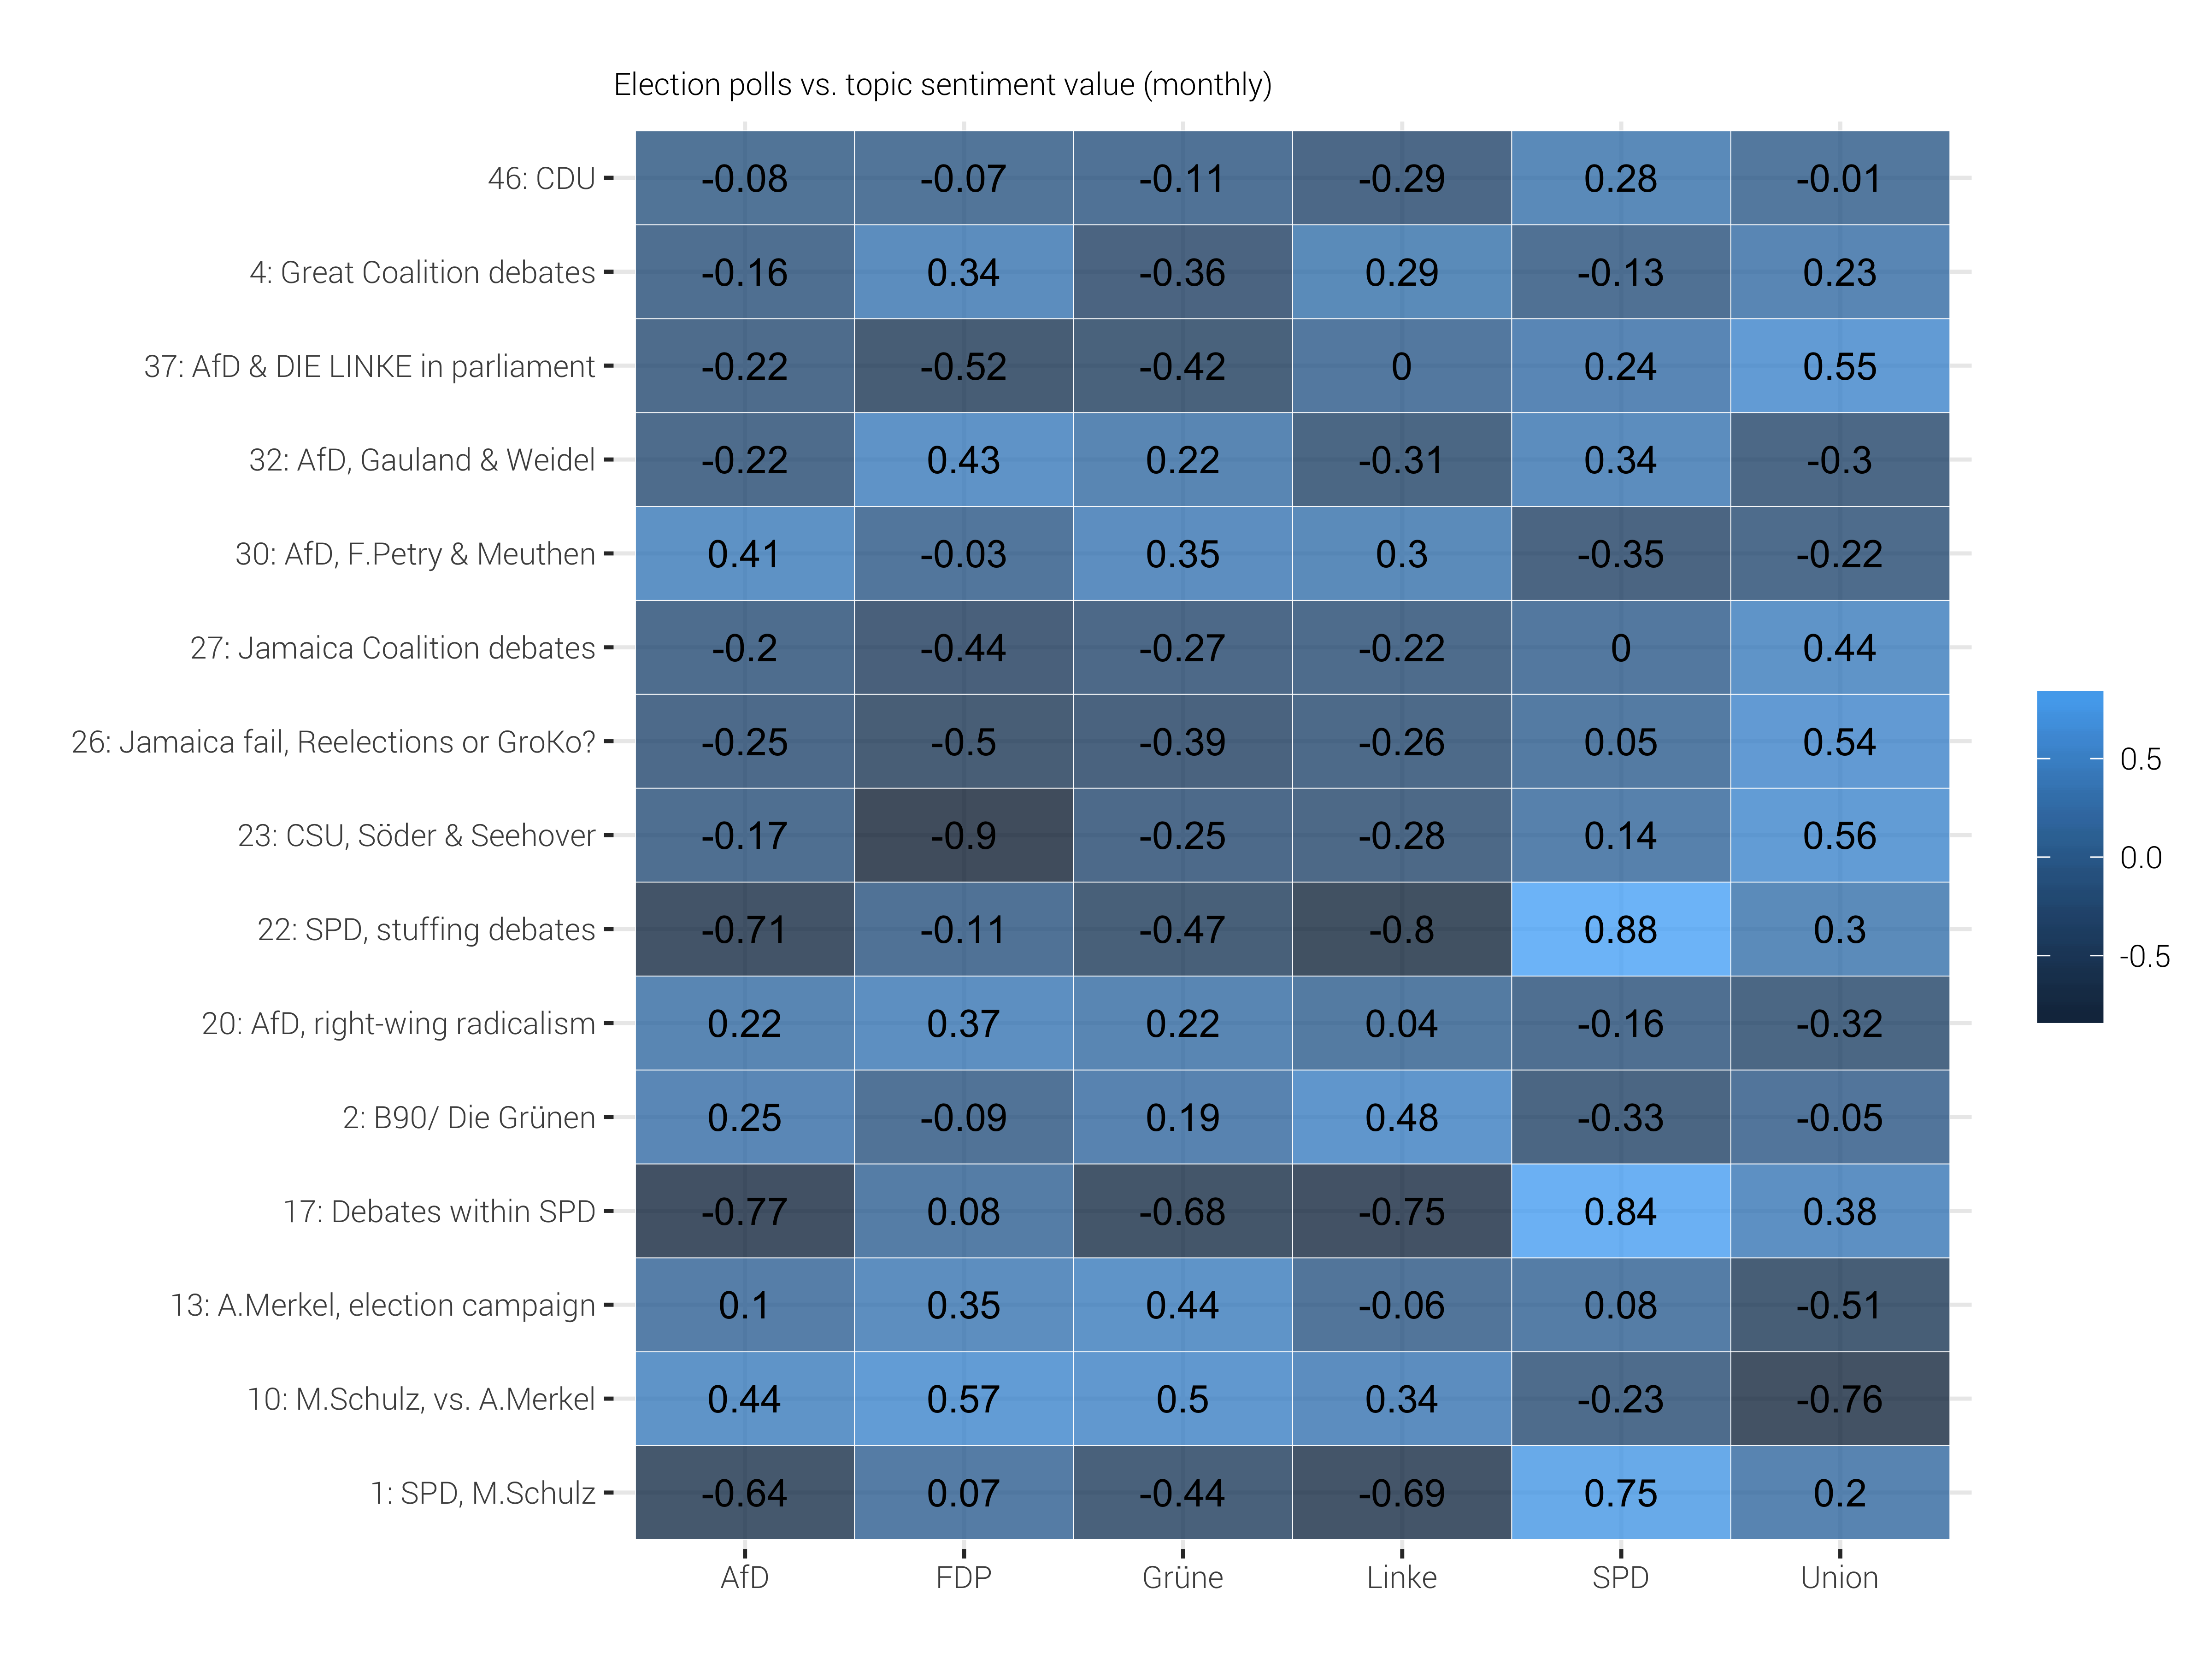
\includegraphics[width=\textwidth,keepaspectratio]{../figs/ccf.png}
			\label{fig_ccf}
	\end{center}
\end{figure}
% Anders darstellen. 
% Eventuell auch Lags zeigen. 

These results suggest that there is a link between the way parties are reported and the political trends within the population. It is obvious to assume that media reporting influences the electorate in its opinion-forming, even if this cannot be proven in this analysis. 

\section{Conclusion}

The purpose of this paper was to examine (1) whether the political reporting of different content providers distinguishes itself and (2) whether this reporting has an influence on the opinion-forming process of the voters. Regarding (1) the analysis revealed that there are differences between the media considered, both in terms of topic prevalence and the way in which these topics are discussed. Although the issues are discussed negatively overall, there are still differences, especially regarding to the coalition negotiations. The smallest differences can be found for topic concerning the AfD. With regard to (2), the analysis has shown that the tonality of topics discussed by the SPD shows a strong positive correlation to current survey results. For CDU/CSU, issues relating to the various coalition negotiations tend to correlate positively with the survey results.  Overall, there seems to be a link between reporting on political issues and electoral preferences. Further research should focus on the exact causal relationships between these two concepts. 

\section*{Appendix}

% 1, 2
\begin{figure}[H]
	\begin{center}
		\begin{subfigure}[normla]{0.49\textwidth}
			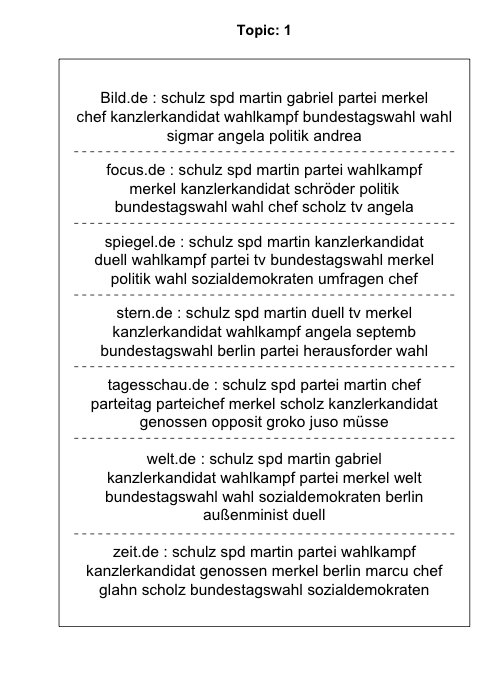
\includegraphics[width=\textwidth]{../figs/plotquote1.png}
		\end{subfigure}
		\begin{subfigure}[normla]{0.49\textwidth}
			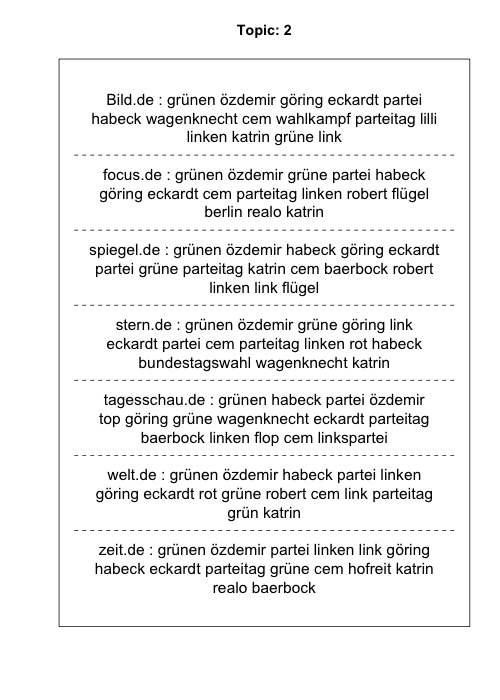
\includegraphics[width=\textwidth]{../figs/plotquote2.png}
		\end{subfigure}
	\end{center}
\end{figure}
	
% 4, 10
\begin{figure}[H]
	\begin{center}
		\begin{subfigure}[normla]{0.49\textwidth}
			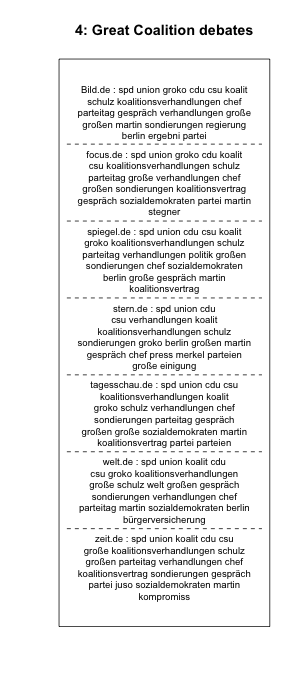
\includegraphics[width=\textwidth]{../figs/plotquote4.png}
		\end{subfigure}
		\begin{subfigure}[normla]{0.49\textwidth}
			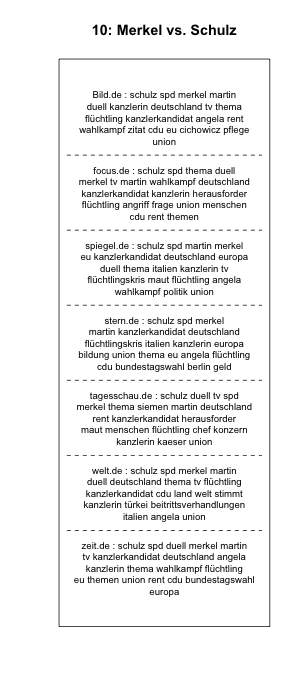
\includegraphics[width=\textwidth]{../figs/plotquote10.png}
		\end{subfigure}
	\end{center}
\end{figure}

% 13, 17
\begin{figure}[H]
	\begin{center}
		\begin{subfigure}[normla]{0.49\textwidth}
			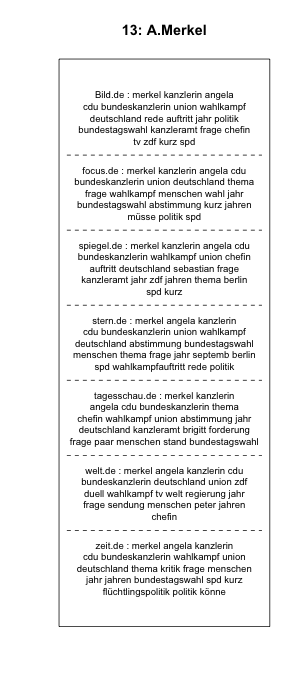
\includegraphics[width=\textwidth]{../figs/plotquote13.png}
		\end{subfigure}
		\begin{subfigure}[normla]{0.49\textwidth}
			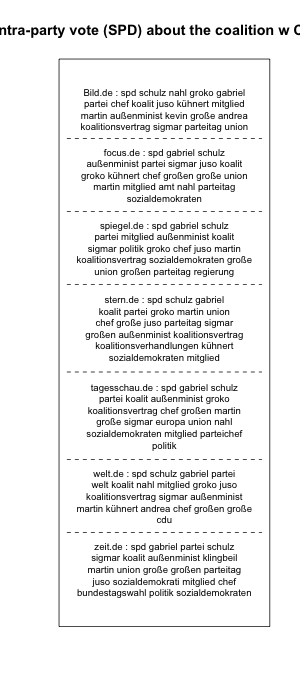
\includegraphics[width=\textwidth]{../figs/plotquote17.png}
		\end{subfigure}
	\end{center}
\end{figure}

% 20, 23
\begin{figure}[H]
	\begin{center}
		\begin{subfigure}[normla]{0.49\textwidth}
			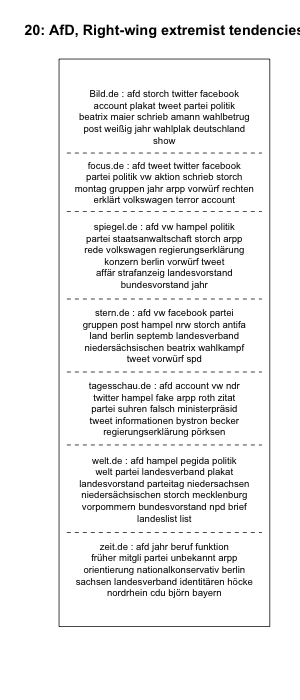
\includegraphics[width=\textwidth]{../figs/plotquote20.png}
		\end{subfigure}
		\begin{subfigure}[normla]{0.49\textwidth}
			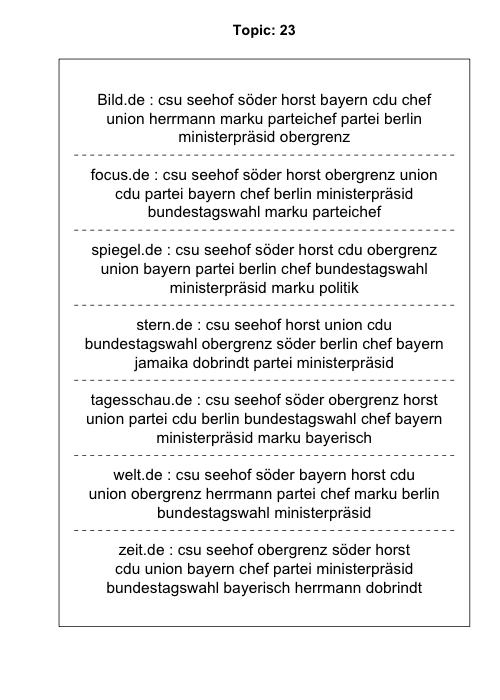
\includegraphics[width=\textwidth]{../figs/plotquote23.png}
		\end{subfigure}
	\end{center}
\end{figure}

% 26, 27
\begin{figure}[H]
	\begin{center}
		\begin{subfigure}[normla]{0.49\textwidth}
			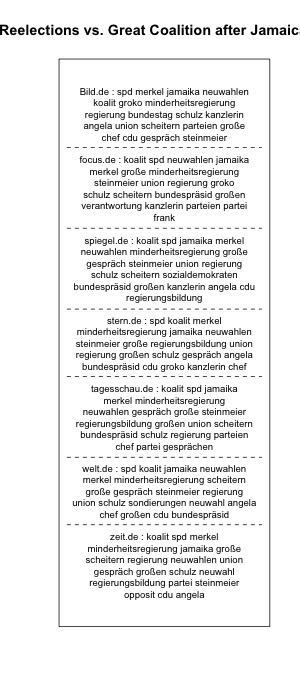
\includegraphics[width=\textwidth]{../figs/plotquote26.png}
		\end{subfigure}
		\begin{subfigure}[normla]{0.49\textwidth}
			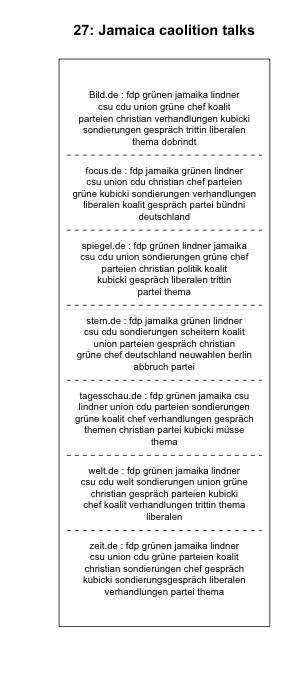
\includegraphics[width=\textwidth]{../figs/plotquote27.png}
		\end{subfigure}
	\end{center}
\end{figure}

% 30, 32
\begin{figure}[H]
	\begin{center}
		\begin{subfigure}[normla]{0.49\textwidth}
			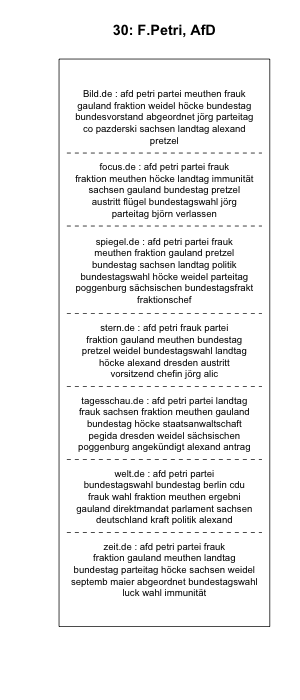
\includegraphics[width=\textwidth]{../figs/plotquote30.png}
		\end{subfigure}
		\begin{subfigure}[normla]{0.49\textwidth}
			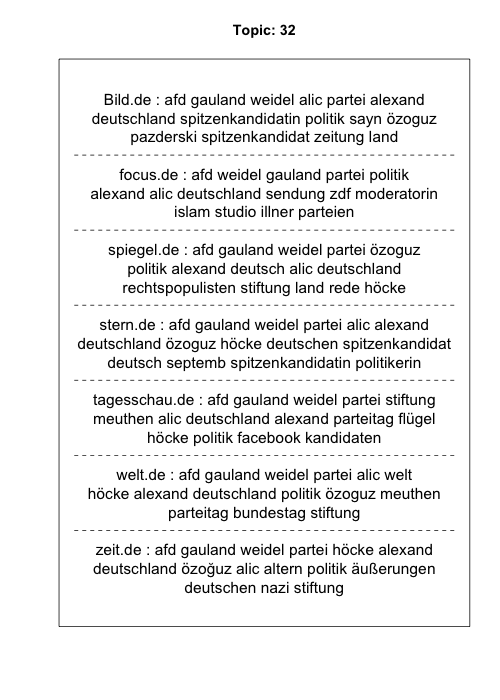
\includegraphics[width=\textwidth]{../figs/plotquote32.png}
		\end{subfigure}
	\end{center}
\end{figure}

% 37, 46
\begin{figure}[H]
	\begin{center}
		\begin{subfigure}[normla]{0.49\textwidth}
			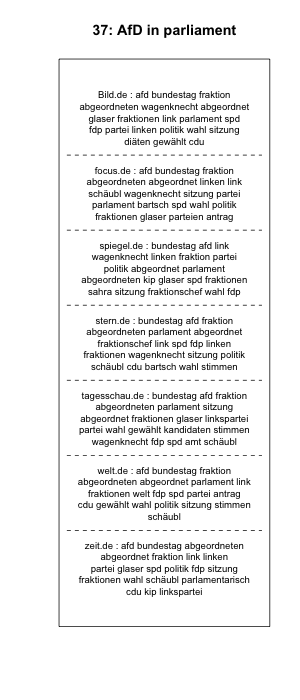
\includegraphics[width=\textwidth]{../figs/plotquote37.png}
		\end{subfigure}
		\begin{subfigure}[normla]{0.49\textwidth}
			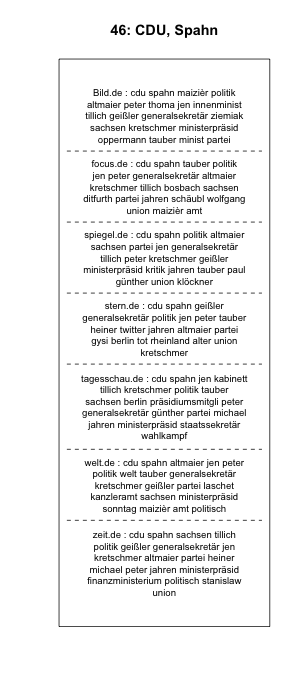
\includegraphics[width=\textwidth]{../figs/plotquote46.png}
		\end{subfigure}
	\end{center}
\end{figure}



\end{document}
